\documentclass{article}
% 数学公式
\usepackage{amsmath}
% 超链接
\usepackage[colorlinks,linkcolor=blue]{hyperref}
\usepackage{url}
\def\UrlBreaks{\do\A\do\B\do\C\do\D\do\E\do\F\do\G\do\H\do\I\do\J
\do\K\do\L\do\M\do\N\do\O\do\P\do\Q\do\R\do\S\do\T\do\U\do\V
\do\W\do\X\do\Y\do\Z\do\[\do\\\do\]\do\^\do\_\do\`\do\a\do\b
\do\c\do\d\do\e\do\f\do\g\do\h\do\i\do\j\do\k\do\l\do\m\do\n
\do\o\do\p\do\q\do\r\do\s\do\t\do\u\do\v\do\w\do\x\do\y\do\z
\do\.\do\@\do\\\do\/\do\!\do\_\do\|\do\;\do\>\do\]\do\)\do\,
\do\?\do\'\do+\do\=\do\#} 

% 代码块
\usepackage{listings}
\usepackage{xcolor}
\lstset{ 
    language = Python,
    backgroundcolor = \color{yellow!10},% 背景色:淡黄
    basicstyle = \small\ttfamily,       % 基本样式 + 小号字体
    rulesepcolor= \color{gray},         % 代码块边框颜色
    breaklines = true,                  % 代码过长则换行
    numbers = left,                     % 行号在左侧显示
    numberstyle = \small,               % 行号字体
    keywordstyle = \color{blue},        % 关键字颜色
    commentstyle =\color[rgb]{0,0.6,0},    % 注释颜色
    stringstyle = \color{red!100},      % 字符串颜色
    frame = shadowbox,                  % 用(带影子效果)方框框住代码块
    showspaces = false,                 % 不显示空格
    columns = fixed,                    % 字间距固定
}

\usepackage{float}
% 加图片 包
\usepackage{graphicx}
\usepackage{subfigure}

% 中文包
\usepackage{xeCJK}
% 控制首行缩进
\usepackage{indentfirst}
\setlength{\parindent}{2em}
% 行间距
\linespread{1.5}

\title{Learning Report}
\author{Bingnan Guo}
\date{July 2021}

\begin{document}
% 生成title
\maketitle
% list the contents

\tableofcontents
% 生成图目录 \listoffigures
\newpage

% --------------------------- SECTION1 ---------------------------
\section{Regression and Classification}
\indent 首先学习的是回归(regression)与分类(classification),以及相关训练过程中的优化方法,图1是一个machine learning的基本框架,给定训练数据(包含输入与标签),需要拟合一个函数(模型),并通过相应的损失函数来约束监督拟合的函数。\par
% Display the figure
\begin{figure}[H]
    \centering
    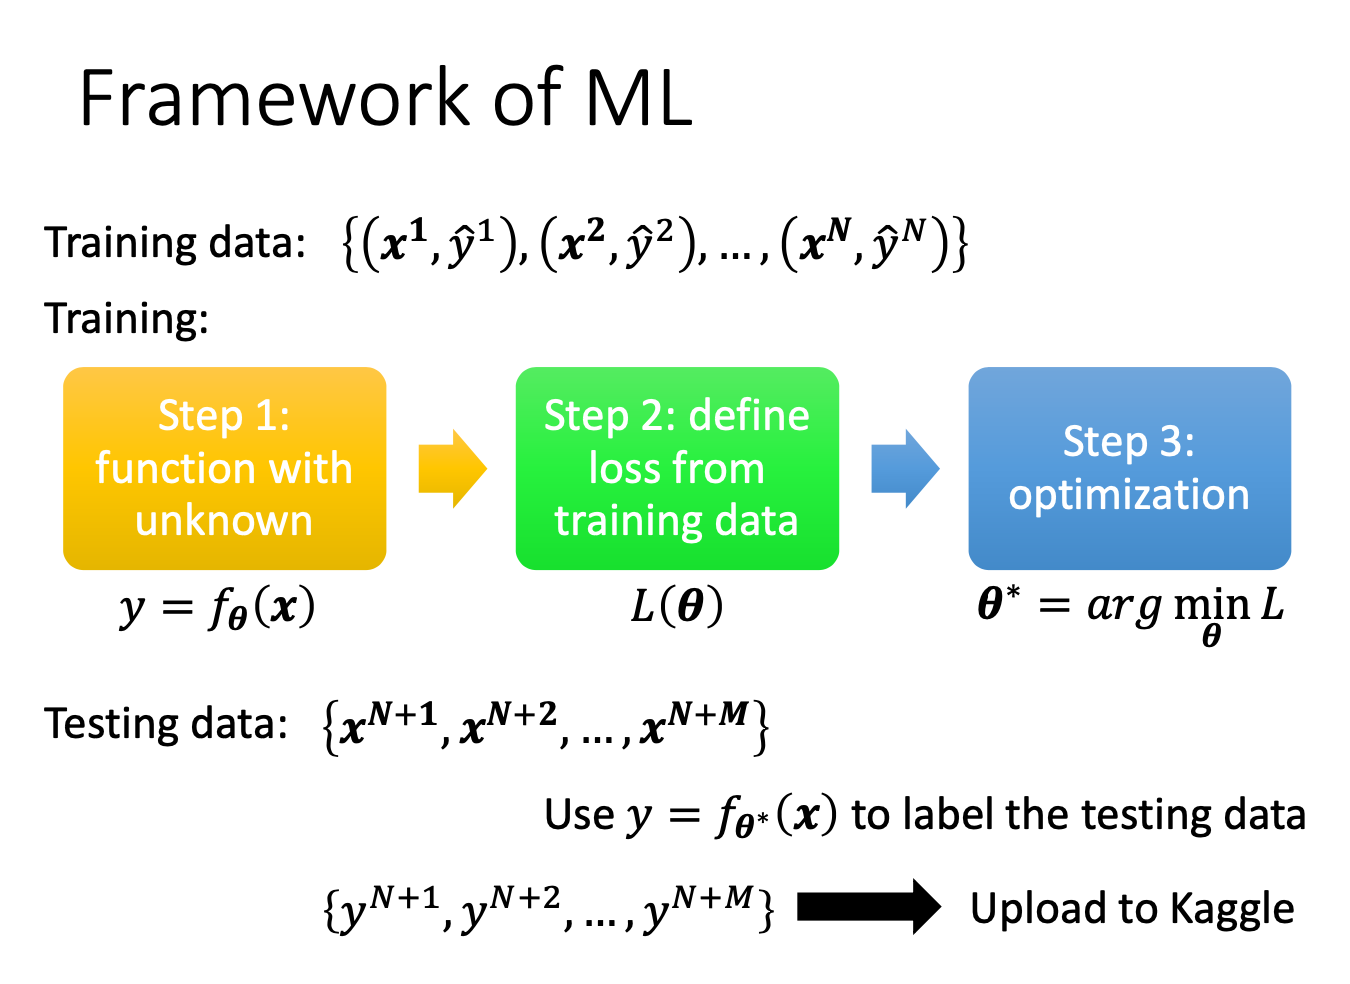
\includegraphics[width=7cm]{picture/FoM.png}
    \caption{Framework of Machine Learning}
    \label{fig:galaxy}
\end{figure}
\indent 对于回归与分类,主要是输出类型不同,回归任务输出一串连续的值,而分类任务中主要输出类别。在一开始的时候,我一直没搞清楚为什么逻辑回归的输出是不连续的0 1,但却是属于回归,但其实该任务本质上属于二分类问题。并且在回归与分类问题中,损失函数也往往不同,在回归任务中,常用的有均方误差(MSE)、平均绝对误差(MAE),在分类任务中,主要有二值交叉熵(Binary Cross Entropy)和交叉熵(Cross Entropy)等。
\begin{figure}[H]
    \centering
    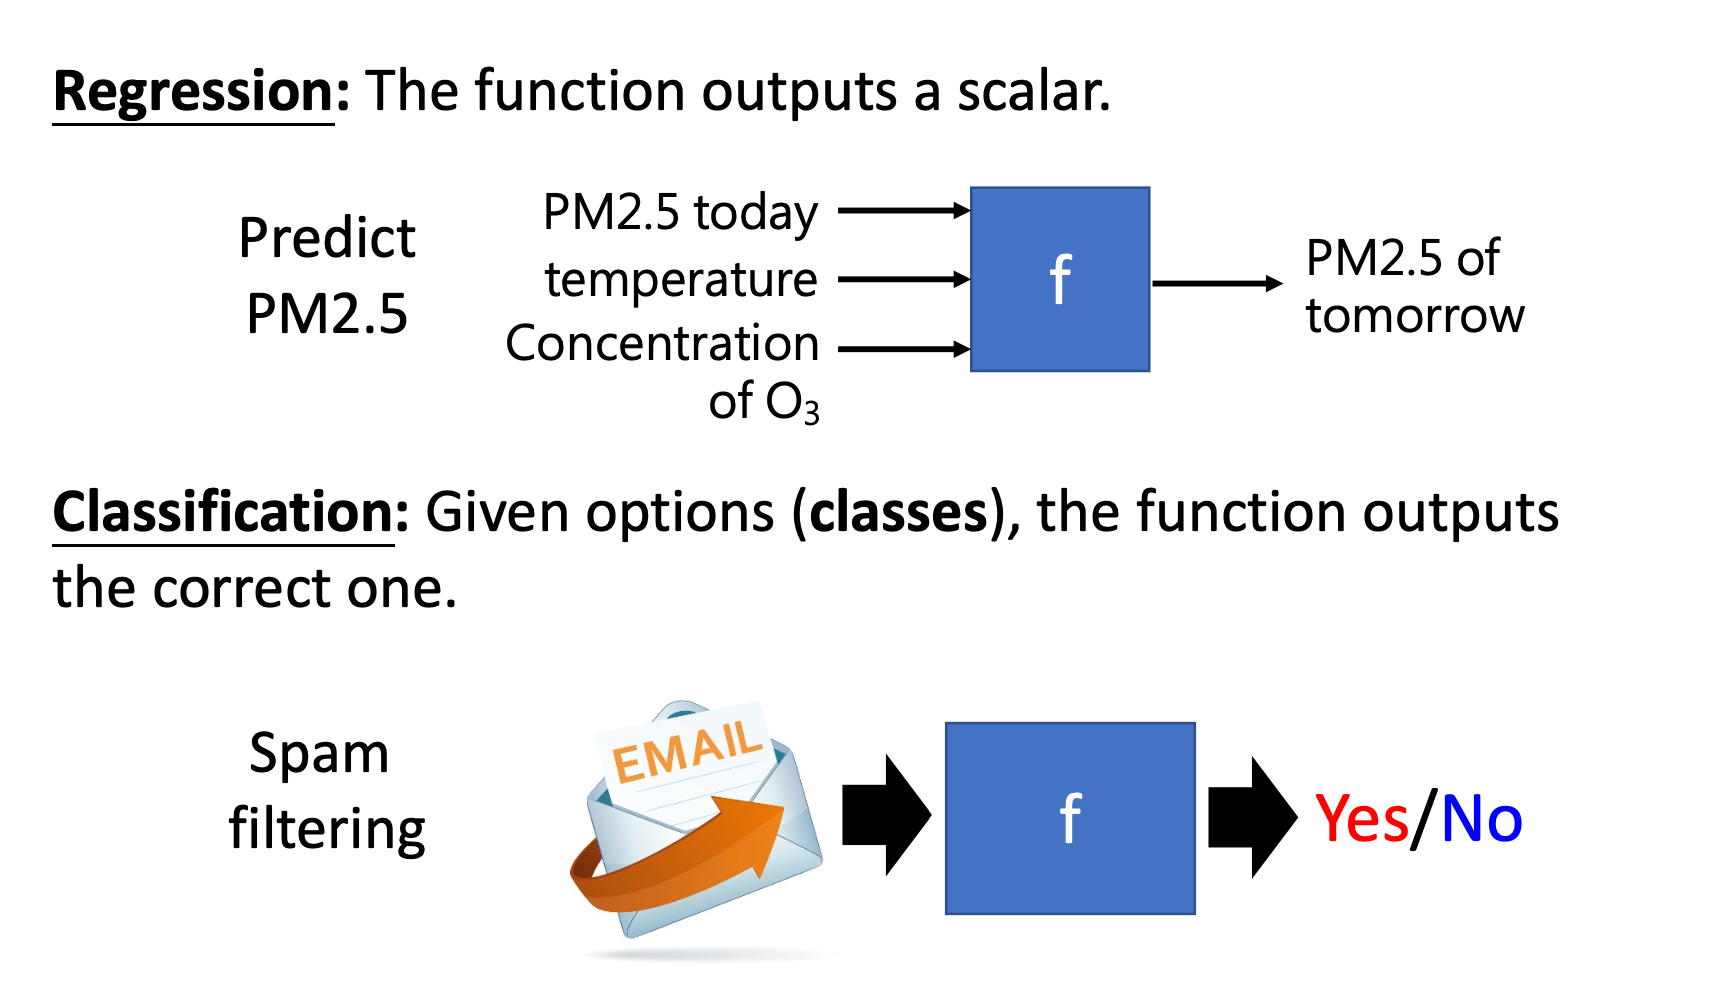
\includegraphics[width=7cm]{picture/RnC1.png}
    \caption{Regression and Classifaction}
    \label{fig:galaxy}
\end{figure}

\begin{figure}[H]
    \centering
    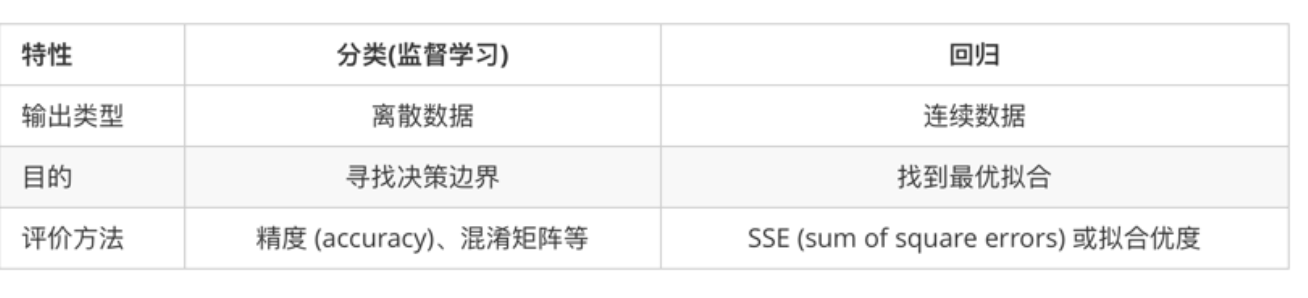
\includegraphics[width=9cm]{picture/RnC.png}
    \caption{Regression and Classifaction2}
    \label{fig:galaxy}
\end{figure}
\indent 在定义了任务类型以及损失函数后,较为重要的就是如何去拟合参数来使得我们定义的损失函数最小,其中梯度下降(Gradient Descent)是极为重要的方法。并给出其公式。
% add equation
\begin{equation}
    \theta = \theta - \alpha \frac{\partial L}{\partial \theta}
\end{equation}

\begin{figure}[H]
    \centering
    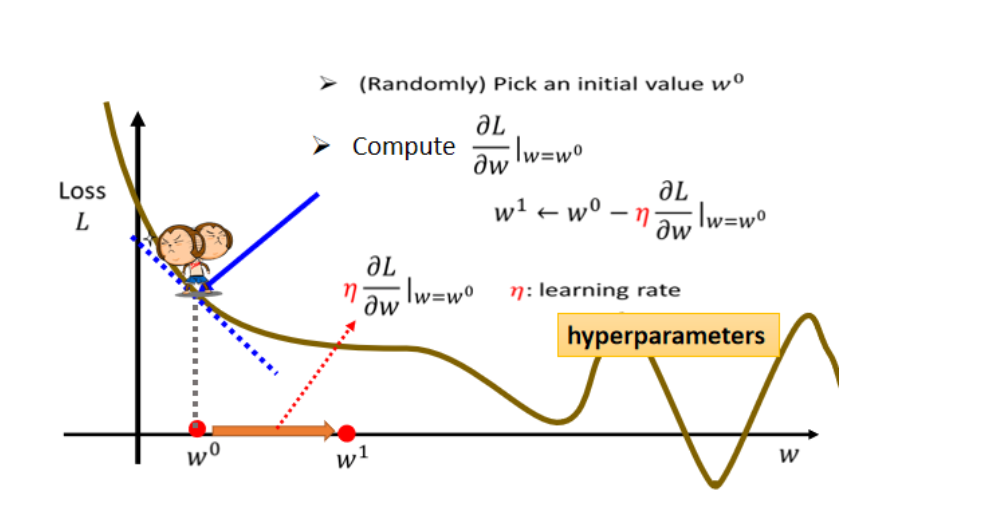
\includegraphics[width=9cm]{picture/grd.png}
    \caption{gradient descent}
    \label{fig:galxy}
\end{figure}
\indent 在梯度下降之后,一个较为重要的概念则是反向传播(Back propagation),我们都知道在计算loss并使用梯度下降的过程中,首先初始化参数,并计算损失函数对各个参数的偏导来完成梯度下降,反向传播主要根据链式法则求导来加快偏导的计算。因此在梯度下降的过程中,首先使用前向传播,将得到的参数放入内存中,再使用反向传播,计算对各个参数的梯度,最后完成梯度下降,最后给出反向传播的链式法则公式及示意图。

\begin{equation}
    \frac{\partial L}{\partial \theta} = \frac{\partial L}{\partial z} \times \frac{\partial z}{\partial \theta}
\end{equation}

\begin{figure}[H]
    \centering
    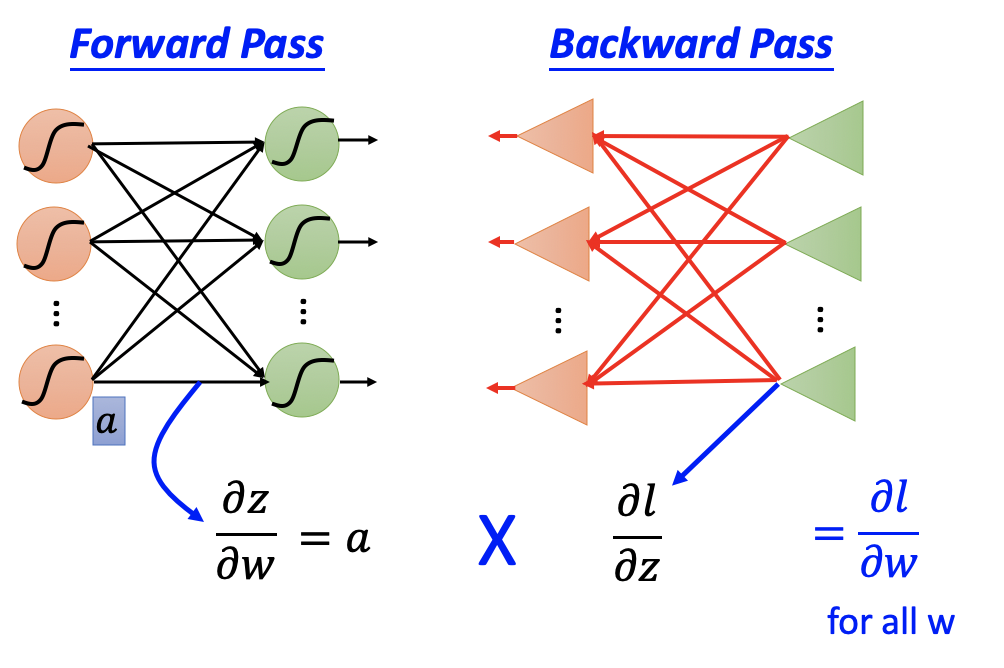
\includegraphics[width=9cm]{picture/Back.png}
    \caption{Back propagation}
    \label{fig:galxy}
\end{figure}

\subsection{Regression}
\indent 在回归任务中,可以通过线性回归来引出神经网络模型。对于简单的线性模型,我们可以拟合少量参数来完成线性回归,但实际上,线性模型相对来说会比较复杂,如图6所示。因此我们需要考虑如何拟合稍复杂的模型,以图6的红曲线为例,该曲线可以看成常数加上蓝色的函数曲线。\par
\begin{figure}[H]
    \centering
    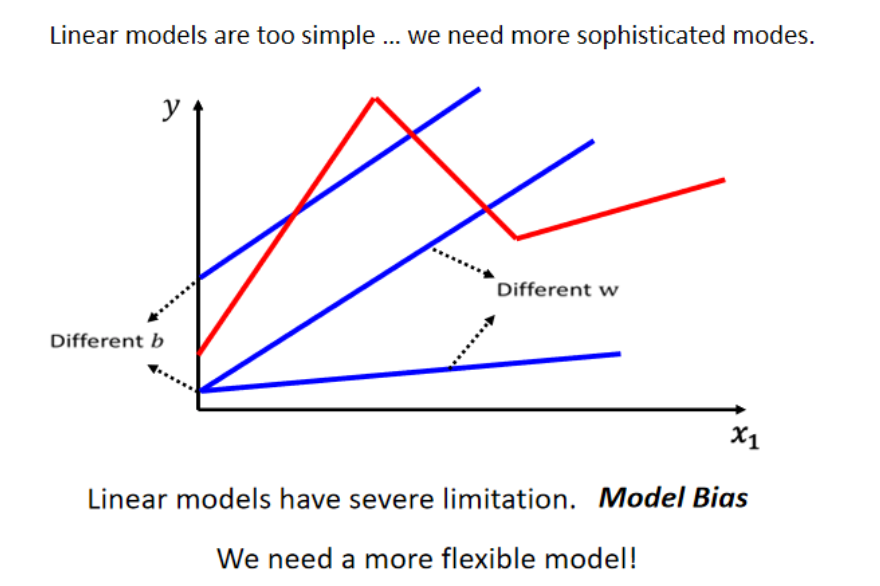
\includegraphics[width=7cm]{picture/LinerModel.png}
    \caption{Different LinerModel}
    \label{fig:galxy}
\end{figure}
\indent 因此在图7中,将稍微复杂的红色曲线表示为多条蓝色曲线以及常数项的叠加,那么如果是更加复杂的线形曲线,我们也同样可以找到多种不同的蓝色曲线,然后叠加常数项得到。\par
\begin{figure}[H]
    \centering
    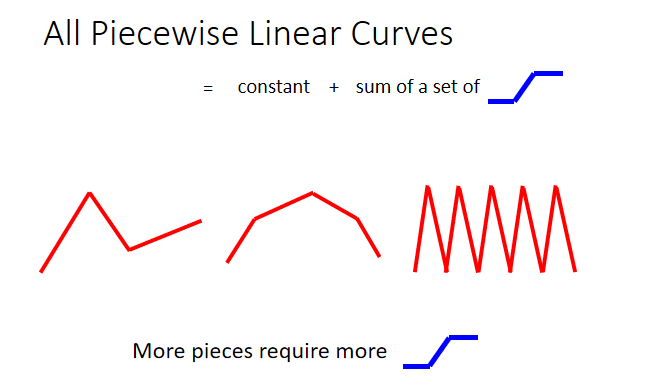
\includegraphics[width=8cm]{picture/LinearCurves.png}
    \caption{Different Linear Curves}
    \label{fig:galxy}
\end{figure}
\indent 我们都知道一条曲线可以由多个线性函数拟合而成,即将曲线分为一小段一小段,然后用线段拟合,因此就可以使用曲线来逼近任意函数,那么我们通常用sigmoid函数来表示最开始的蓝色曲线函数。sigmoid函数的具体形式如公示3所示。\par
\begin{equation}
    y = c \frac{1}{1 + e^{-(b + wx_{1})}}
\end{equation}
\begin{figure}[H]
    \centering
    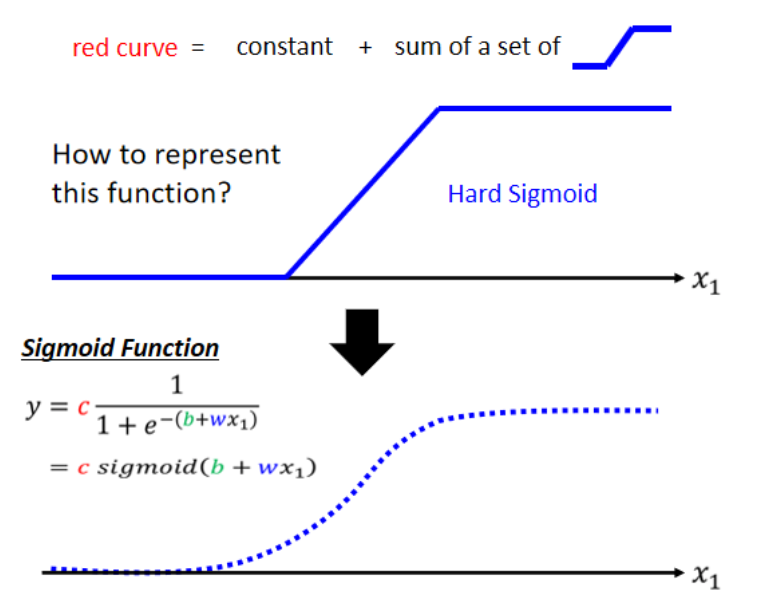
\includegraphics[width=8cm]{picture/Sigmoid.png}
    \caption{Sigmoid}
    \label{fig:galxy}
\end{figure}
\indent 通过调整sigmoid的不同参数,我们可以拟合不同的曲线,为了使得我们的函数能够表达更多不同的曲线,给出如下的公式:
\begin{gather*}
    y = b + \sum_{i} c_{i} sigmoid ( b_{i} + w_{i} x_{i})  \\
    y = b + \sum_{i} c_{i} sigmoid \left( b_{i} + \sum_{j} w_{ij} x_{i} \right)
\end{gather*}
\indent 在上述公式中,假设i、j为1 2 3,那么将表达式列举出来,具体如图9所示,可以发现sigmoid中可以表示为r=b+wx的,那么就相当于经过线性变化再通过sigmoid函数。
\begin{figure}[H]
    \centering
    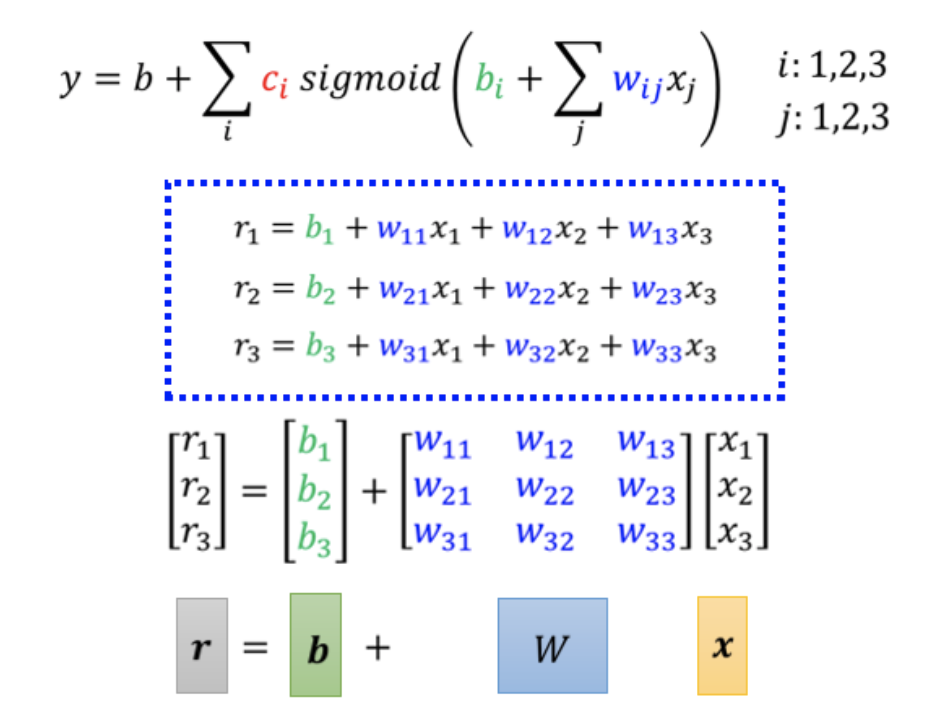
\includegraphics[width=8cm]{picture/EepofSig.png}
    \caption{Explanation of Sigmoid function}
    \label{fig:galxy}
\end{figure}
\indent 因此我们就可以得到一个简单的神经网络模型,输入向量经过线性变化,再经过sigmoid激活函数以及最后的线形变化得到输出,构成了一个极其简单的网络模型。
\begin{figure}[H]
    \centering
    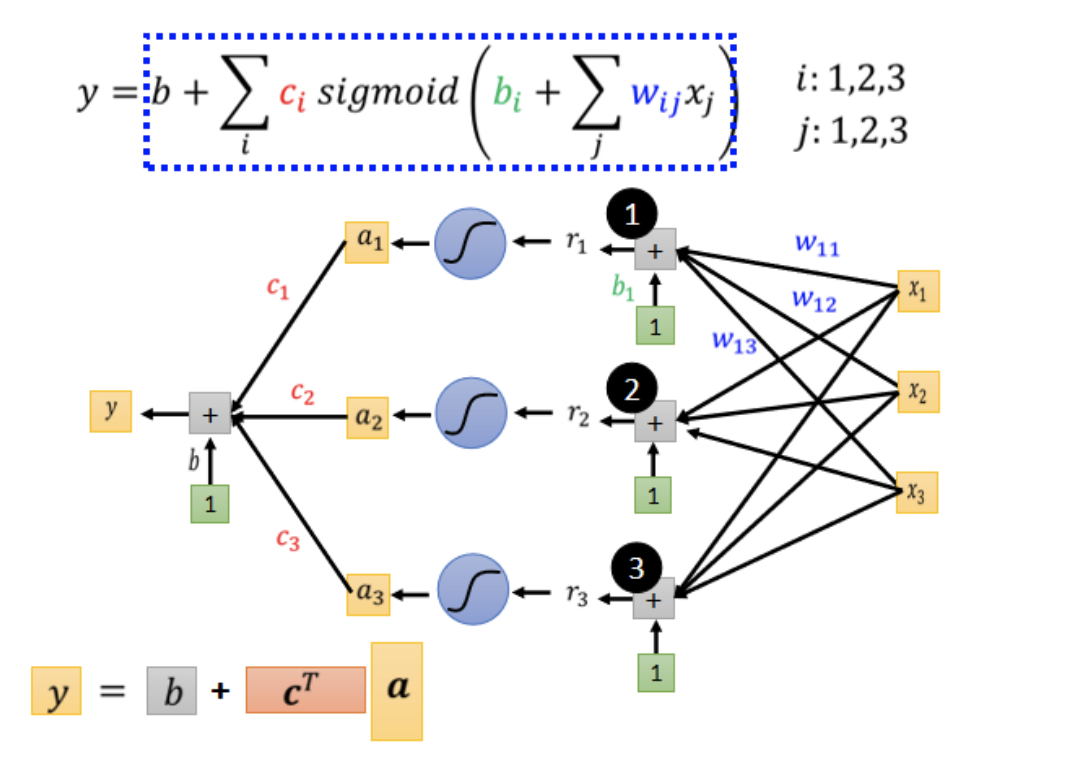
\includegraphics[width=8cm]{picture/LtoNN.png}
    \caption{simple neural network}
    \label{fig:galxy}
\end{figure}
\indent 在网络模型中,激活函数通常使用Relu,而在本节的Regulation中,主要叙述了从线性模型引出基本神经网络模型,这是该课程以独特的角度为我们介绍神经网络模型,因此我们能从不同的角度理解神经网络的构成。
\newpage

\subsection{Classifaction}
\indent 简单来说,分类任务是输入一些向量(可以是表示图像、文字序列的向量),然后输出\( \hat{y} \),可以使用固定的数字来表示类别,但是在分类任务中,更多的使用one-hot向量来表示,具体如下所示,三个向量分别表示class1、class2、class3。
\begin{align*}
    \hat{y}&=\begin{bmatrix}
            1\\
            0\\
            0
    \end{bmatrix} or  & 
    \hat{y}&=\begin{bmatrix} 
            0\\
            1\\
            0
    \end{bmatrix} or &
    \hat{y}&= \begin{bmatrix}
            0\\
            0\\
            1
    \end{bmatrix}
\end{align*}
\indent 但是在分类的过程中,往往会将神经网络输出的y再通过Soft-max的function得到y',然后才去计算loss,至于加上Soft-max的原因,一个比较简单的解释是我们所表示类别的One-hot向量中表示的的值只有0和1,而神经网络输出的有任何值,所以通过Soft-max层将其标准化为0,1。
\begin{figure}[H]
    \centering
    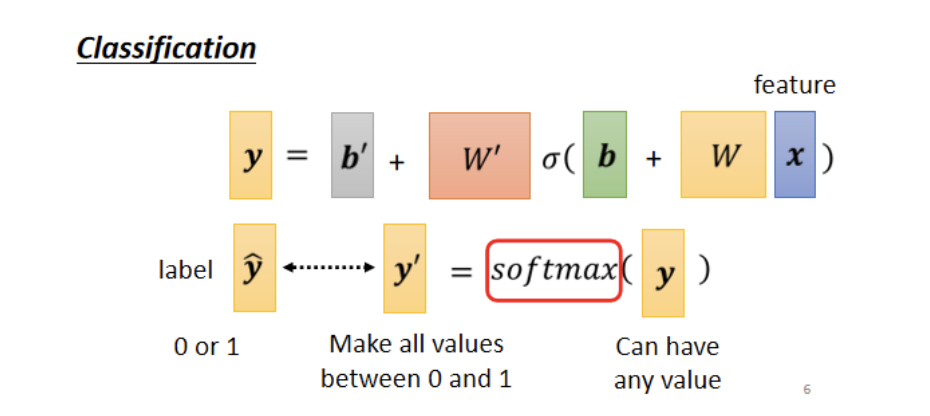
\includegraphics[width=8cm]{picture/Classify.png}
    \caption{Classification}
    \label{fig:galxy}
\end{figure}
\indent 因此将会初步的介绍一下Soft-max的运行机制,具体如下图所示。并给出其具体的计算公式。从图中可知,输入任何值,Soft-max函数都会根据权重输出0~1间的数字,因此在后续的数据处理中,我们可以设定阈值,将超出最大的值赋值为1,其他赋值为0,就可以得到预测结果,这点在HW3中的半监督学习法中有所体现。
\begin{equation}
    y^{\prime }_{i}  = \frac{exp(y_{i})}{\sum_{j} exp(y_{j})}
\end{equation}
\begin{figure}[H]
    \centering
    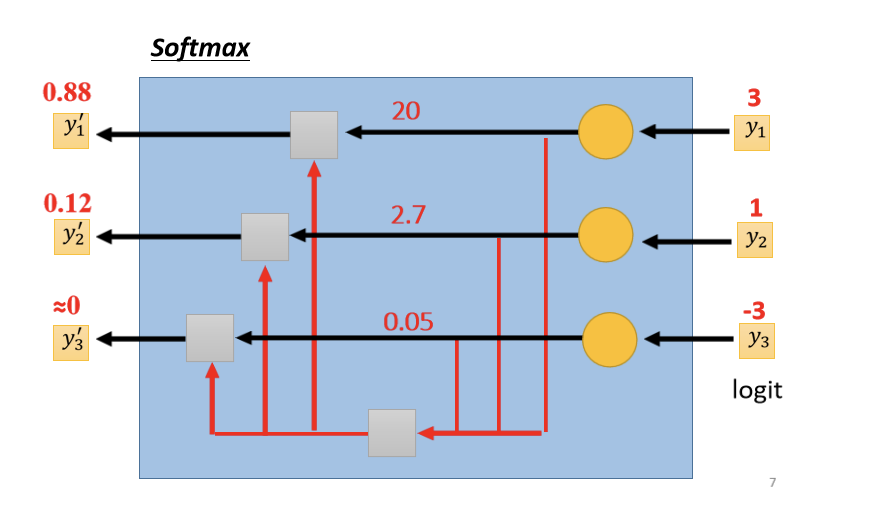
\includegraphics[width=8cm]{picture/softmax.png}
    \caption{Soft-max}
    \label{fig:galxy}
\end{figure}
\indent 在分类任务中,还有一个比较重要的是分类的损失函数,在分类任务中较为常见的是使用Cross-entropy即使用交叉熵损失函数,并给出其公式以及调用方式。
\begin{equation}
    e = - \sum_{i} \hat{y_{i}} ln y^{\prime}_i
\end{equation}

% 代码段
\begin{lstlisting}
# Soft-max的函数定义
torch.nn.functional.softmax(input, dim=None, _stacklevel=3, dtype=None)
# Cross-entropy的函数定义
torch.nn.CrossEntropyLoss(weight: Optional[torch.Tensor] = None, size_average=None, ignore_index: int = -100, reduce=None, reduction: str = 'mean')
\end{lstlisting}

\indent 需要注意的是,在pytorch中Cross-entropy和Soft-max是绑定在一起的,如果你使用了Cross-entropy来计算loss,那么Soft-max将会自动加入你构建神经网络的最后一层。\par
\newpage

\subsection{Optimization}
\indent 紧接着就是在训练过程中遇到问题如何去优化,包括如何根据训练过程中训练数据或者是验证数据的loos来判断你构建的神经网络的性能,是欠拟合还是过拟合?是否需要加深你的网络结构?或者是给更多的数据?又或者是采用正则化以及其他优化器,因此将在图13中给出一个判断网络性能的概览图。
\begin{figure}[H]
    \centering
    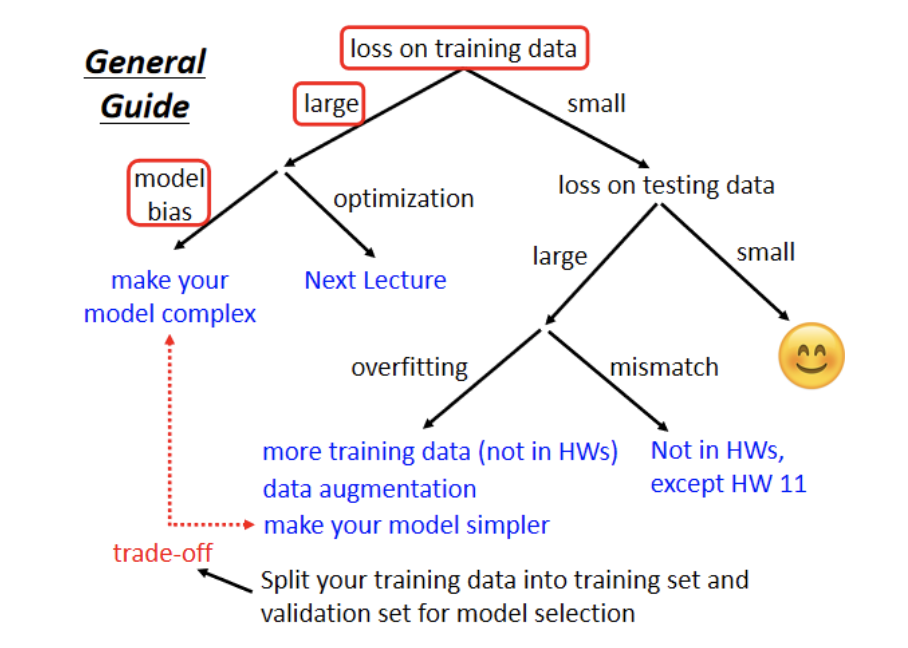
\includegraphics[width=8cm]{picture/General_Guide.png}
    \caption{General Guide}
    \label{fig:galxy}
\end{figure}
\indent 如果在训练数据上发现loss很高,并没有训练好,那么你就需要考虑是什么原因导致,那么会有两个可能,其中一个则是Model bias,即模型的结构设置过于简单。这个时候就需要重新设计模型使得模型具有更大的弹性。当然,在训练数据上loss高的另一个原因则是优化问题,其实梯度下降往往存在着很多问题,接着将会介绍训练策略及优化器。\par
\subsubsection{Batch}
\indent  在下图中,给出了Batch的介绍,在神经网络的训练中,会有一个参数叫batch size,其代表将需要训练的数据分为多个大小为batch size的Batch。所以训练的过程可以概括为,使用一个Batch的数据计算loss,再计算gradient,最后update参数,将所有的Batch训练过一遍则称为一轮Epoch,其中值得注意的是,在每一轮Epoch开始前,会进行Shuffle使得每次Epoch开始前Batch中的数据不同。
\begin{figure}[H]
    \centering
    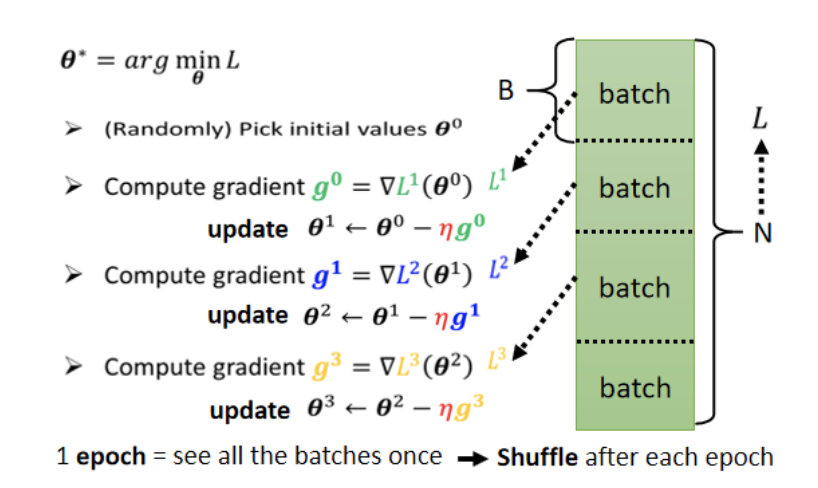
\includegraphics[width=8cm]{picture/Batch.png}
    \caption{optimization with batch}
    \label{fig:galxy}
\end{figure}
\indent 那么不同大小的batch size对性能是否有什么影响,这里引用了在MNIST以及CIFAR-10中的两个实验结果。
\begin{figure}[H]
    \centering
    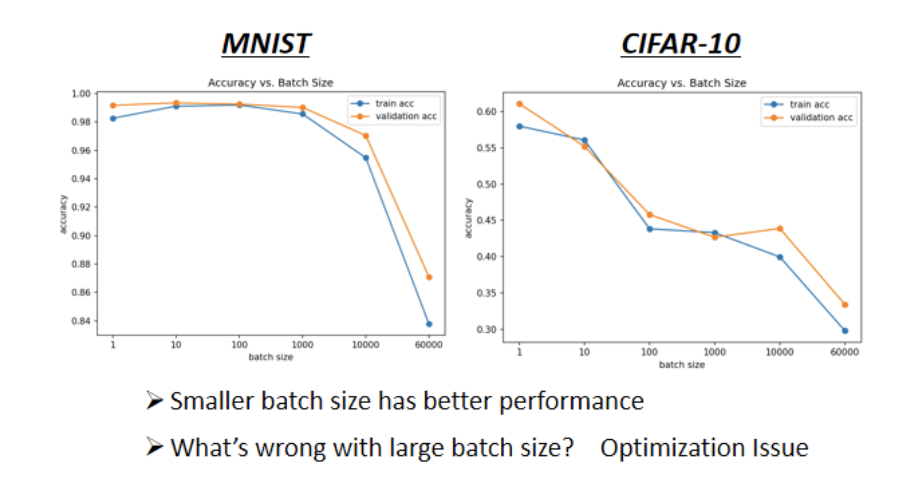
\includegraphics[width=8cm]{picture/DBatch.png}
    \caption{optimization with batch}
    \label{fig:galxy}
\end{figure}
\indent 可以发现极大的batch size的(超过1000)结果并不好,相对来说偏小的batch size(小于1000)有着就好的结果,但是具体的batch size作为一项超参需要在训练过程中根据不同的任务去调整。\par
\newpage

\subsubsection{Momentum}
\indent 接着会介绍几个优化器,可以解决Saddle Point(鞍点)或者Local Minima(局部最小值),首先给出梯度下降+Momentum的公式,其中m为每次迭代需要移动的参数。通过\( \theta \)来计算梯度\( g \)。
\begin{align*}
    m^{0} &= 0 \\
    m^{1} &= \lambda m^{0} -  \eta g^{0}\\
    \theta^{1} &= \theta^{0} + m^{1}\\
    m^{2} &= \lambda m^{1} -  \eta g^{1}\\
    ...&...
\end{align*}

\begin{figure}[H]
    \centering
    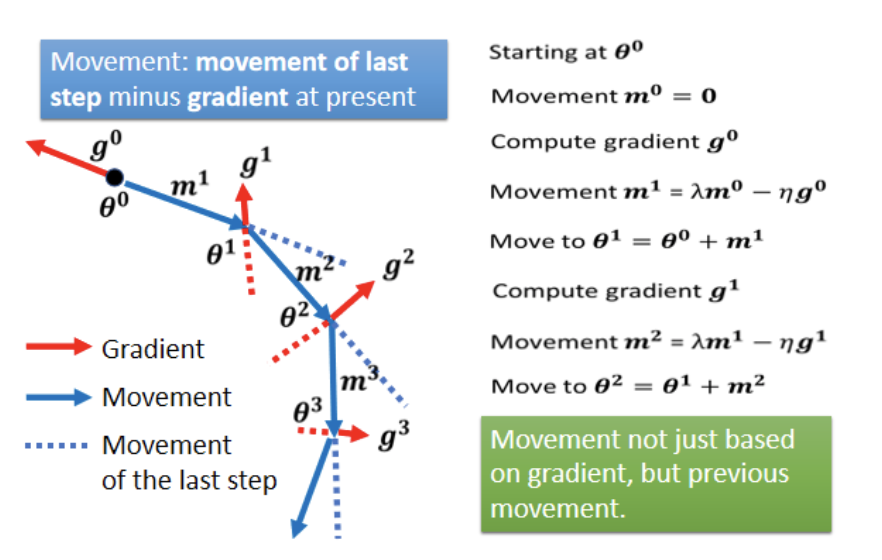
\includegraphics[width=8cm]{picture/Momentum.png}
    \caption{optimization with batch}
    \label{fig:galxy}
\end{figure}
\indent 以此类推,可以发现在梯度下降加上Momentum后,可以表述为梯度的负反方向加上前一次移动的方向。从其他角度看,当加上Momentum的时候,更新参数的方向不是只考虑现在的 梯度,而是考虑过去所有梯度的总和.在pytorch中,Momentum直接被集成到梯度下降函数中,可以直接设定其参数值。
\begin{lstlisting}
# SGD-梯度下降中可以直接使用Momentum设置参数
torch.optim.SGD(params,lr=<required parameter>,
                momentum=0, dampening=0,weight_decay=0, nesterov=False)
\end{lstlisting}
\newpage

\subsubsection{RMSProp and Adam}
\indent 当训练一个神经网络的过程中,训练后发现loss不再下降的时候,可能卡在local minima,也可能卡在saddle point,但有时候根本两个都不是,只是单纯的loss没有办法再下降。\par
\begin{figure}[H]
    \centering
    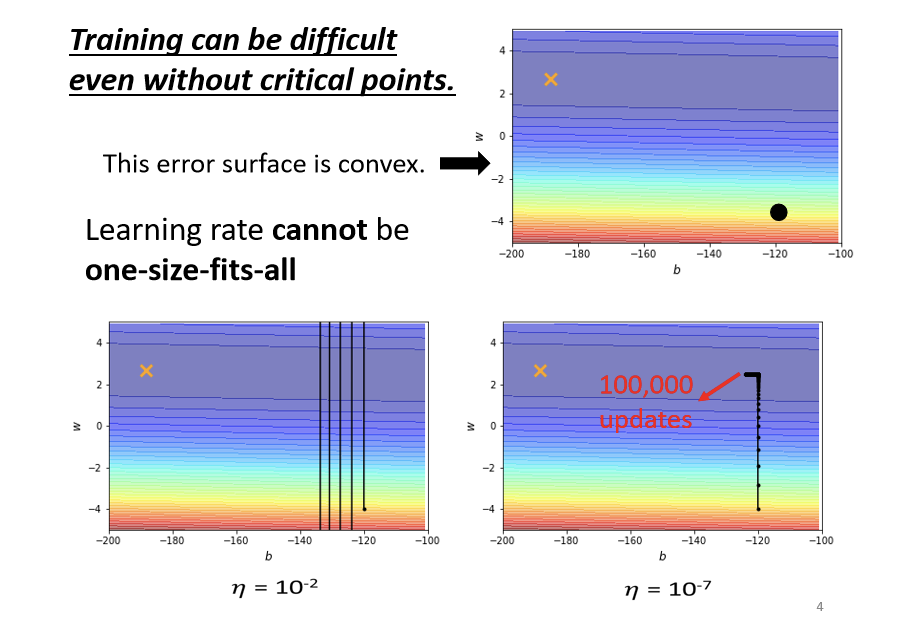
\includegraphics[width=8cm]{picture/TrainingDifficult.png}
    \caption{Why traning loss donot change}
    \label{fig:galxy}
\end{figure}
\indent 在上图中可以简单的可视化训练过程,如果以较大的学习率来训练,可以发现参数不断的在震荡,无法收敛,若以较小的学习率来训练,始终在一个点而无法继续前进,因此这就需要自适应学习率。给出公式。
\begin{equation}
    \begin{split}
     \theta^{t+1}_i \xleftarrow{}\theta^{t}_i - \frac{\eta}{\sigma^{t}_i} g^{t}_i\\
     g^{t}_i = \frac{\partial L}{\partial \theta_{i}} \vert \theta = \theta^{t}
    \end{split}
\end{equation}
\indent 其中\( g^{t}_i\)代表在第t个iteration中的微分,因此就可以不同的参数、迭代次数中会存在不同的学习率,那么接下来则会考虑如何计算这个自适应的学习率。公式如下所示。
\begin{equation}
    \sigma^{t}_{i} = \sqrt{\frac{1}{t+1} \sum^{t}_{i=0} (g^{t}_{i})^{2}}
\end{equation}
\indent 上述公式是被使用于一个叫做Adagrad的方法中,可以能够根据每一次参数梯度的不同来调整学习率的大小,但是在某些情况下,在同一个参数的同一个梯度也需要学习率能够进行动态调整,因此就提出了RMS Prop,具体如下图所示,并给出公式。
\begin{figure}[H]
    \centering
    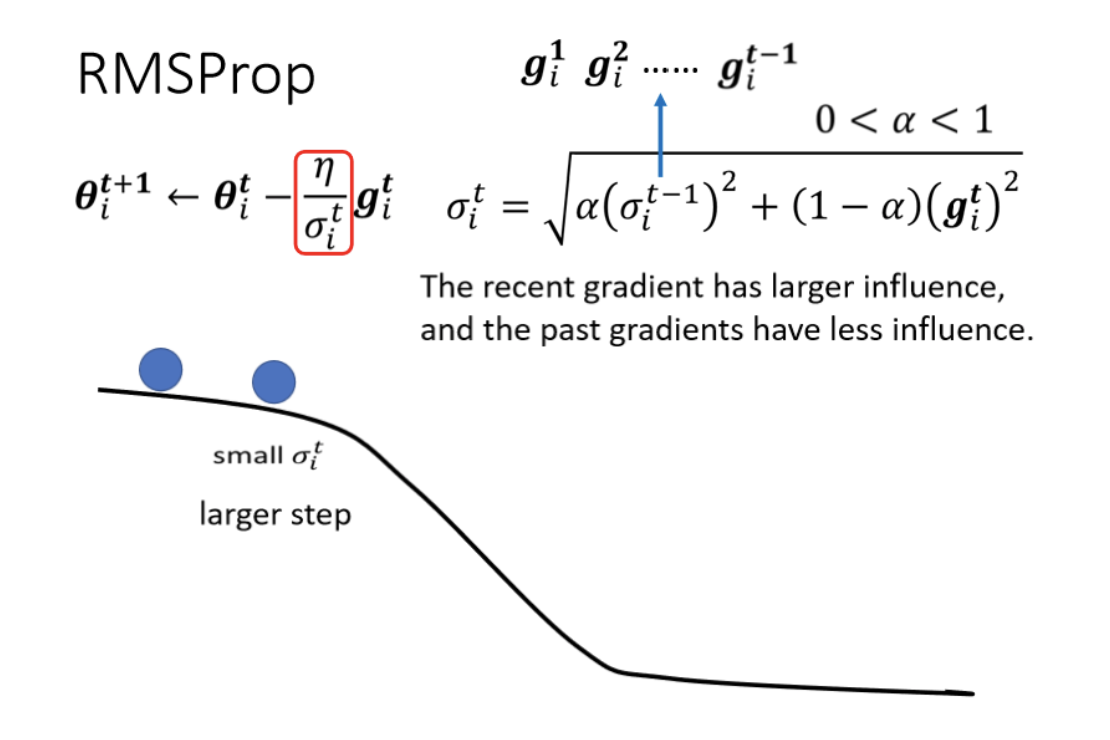
\includegraphics[width=8cm]{picture/RmsProp.png}
    \caption{RMSProp}
    \label{fig:galxy}
\end{figure}
\indent 通过\(\alpha\)这一项可以决定\(g^{t}_{i}\)相较于之前的\(\sigma^{t-1}_{i}\)中的\(g^{t-1}_{i}\)而言,它的重要性有多大,如果使用RMSProp,就可以动态调整\(\sigma\)这一项。
\begin{equation}
    \sigma^{t}_{i}=\sqrt{\alpha(\sigma^{t-1}_{i})_{2} + (1- \alpha)(g^{t}_{i})^{2}}
\end{equation}

\indent 在优化策略中,最常用的就是Adam,Adam中的策略即为RMSProp+Momentum,该优化器在pytorch中可以直接调用。\par
\begin{figure}[H]
    \centering
    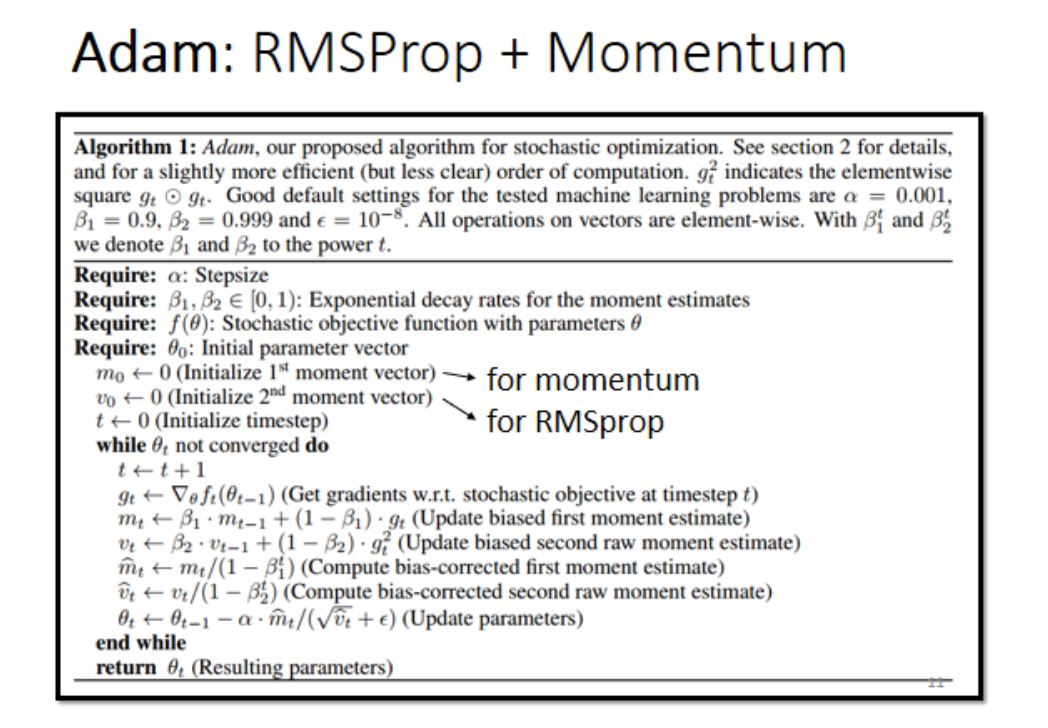
\includegraphics[width=10cm]{picture/Adam.png}
    \caption{the implementation Adam}
    \label{fig:galxy}
\end{figure}

\begin{lstlisting}
# Adam优化器及其初始参数
torch.optim.Adam(params, lr=0.001, betas=(0.9, 0.999), eps=1e-08, weight_decay=0)
\end{lstlisting}
\indent 在上述的公式中我们可以发现\(\eta\)是个固定值,那么考虑以下的情况,如果梯度一直很小,那么就累积了很小的\(\sigma\),当累计的\(\sigma\)足够小,则会忽然变的很大,因此需要一些策略来解决这些问题,即Learning rate Decay与Warm up。\par
\begin{figure}[H]
    \centering
    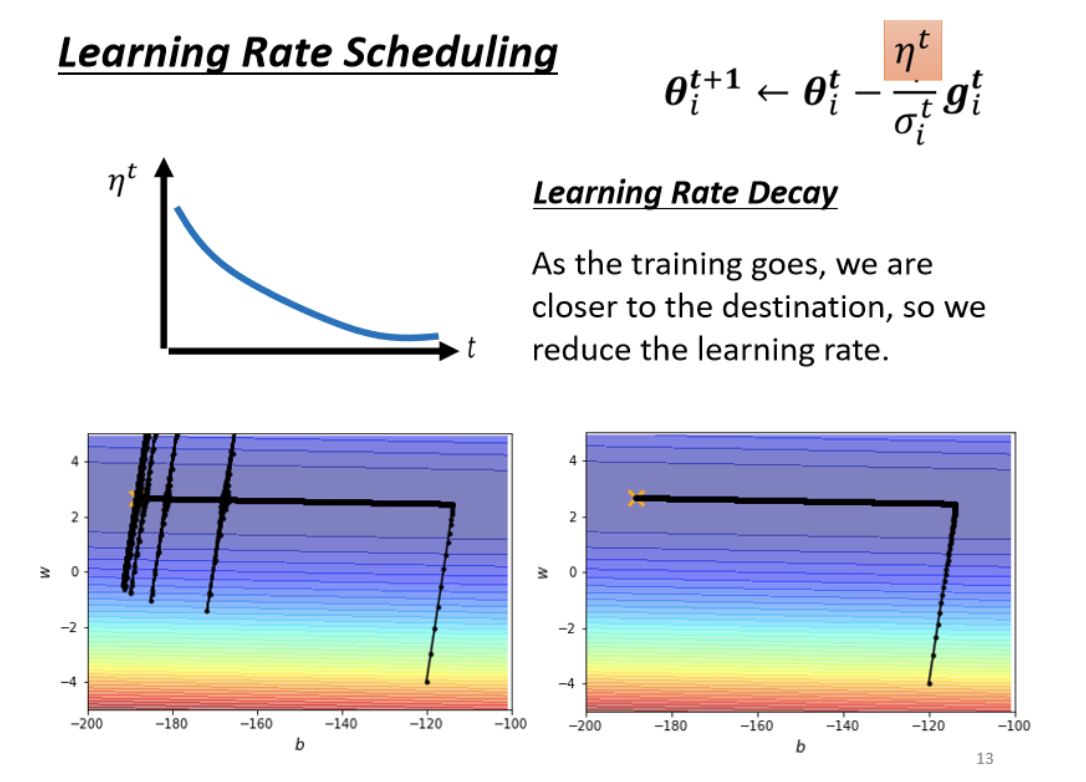
\includegraphics[width=8cm]{picture/WeightDecay.png}
    \caption{WeightDecay}
    \label{fig:galxy}
\end{figure}
\indent Weight Decay是持续让学习率逐步减少,逐渐慢慢变小。\par
\indent Warm Up这个方法是让学习率先变大后变小,具体变小的速度与点是作为超参需要调整,但是总体策略是,学习率要先变大后变小,其往往被ResNet、BERT、Transformer用到。
\begin{figure}[H]
    \centering
    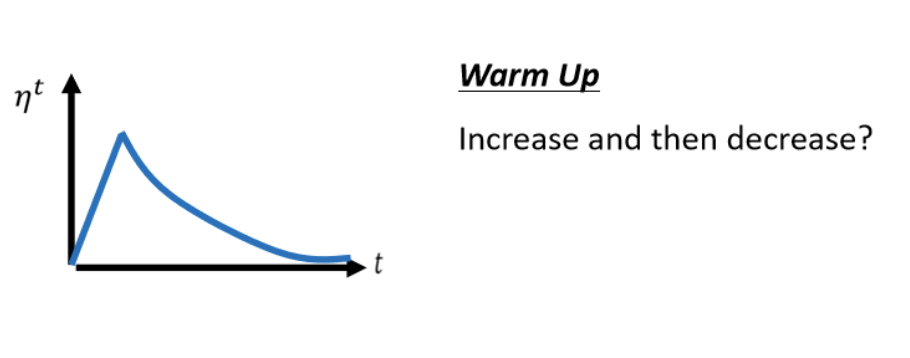
\includegraphics[width=8cm]{picture/Warm-up.png}
    \caption{the implementation Adam}
    \label{fig:galxy}
\end{figure}
\newpage

% -------------------------- 卷积神经网络 SECTION2 ------------------------
\section{Convolutional Neural Network}
\indent 在这一节中,将会记录一下课程中学习的卷积神经网络(Convolutional Neural Network)即CNN,该网络架构主要呗应用于视觉研究领域。在图像分类的任务中,将图片作为输入并输出预测值,较为常见的处理方法是将所有的数据图片Rescale成一样的大小,再放入模型中进行训练预测。我们所期望的输出是一个One-Hot的Vector,包括对类别的预测输出。
\begin{figure}[H]
    \centering
    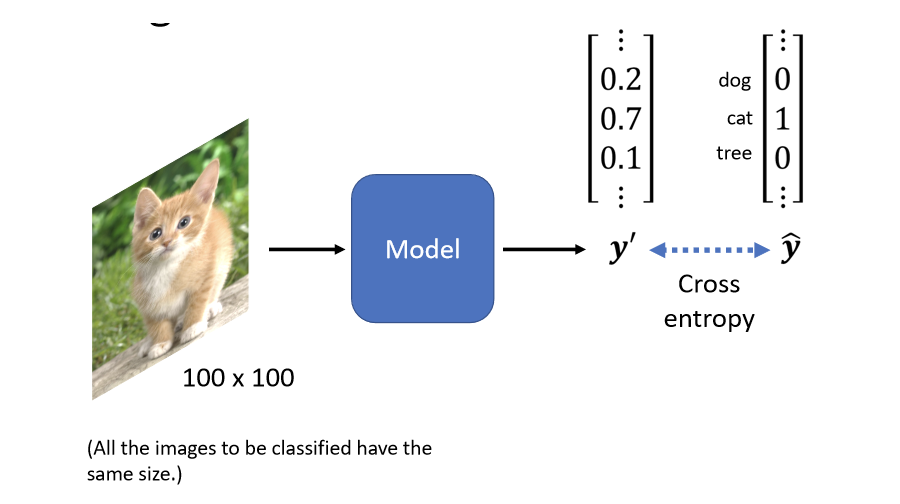
\includegraphics[width=8cm]{picture/ImageClassify.png}
    \caption{Image Classification}
    \label{fig:galxy}
\end{figure}

\indent 那么首先考虑输入,一张图片其实可以看成三维的Tensor,即相当于width*height*channel的Tensor,可以将其进行拼接,转化成一维的Tensor,作为网络的输入。\par
\begin{figure}[H]
    \centering
    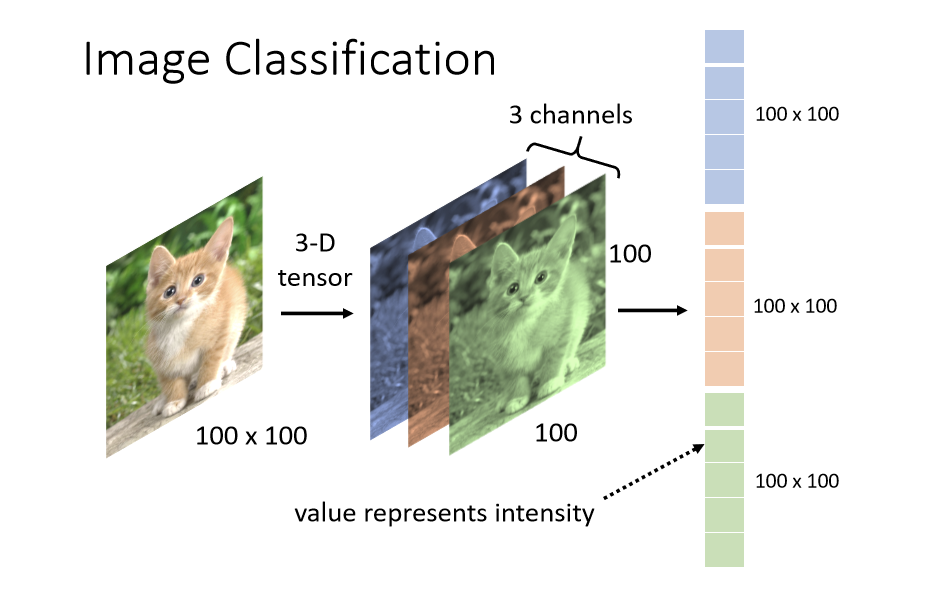
\includegraphics[width=8cm]{picture/ImageClassification.png}
    \caption{Image Classification2}
    \label{fig:galxy}
\end{figure}
\indent 因此可以发现,输入的向量数据非常的多,如果使用全连接层,随着模型层数的增加,可能会增加模型过拟合的风险,因此设计一个比较特别的模型来解决图像分类的问题是比较有意义的。\par
\indent 在图像分类的过程中,我们通常会根据一个动物的相应特征来判断,那么在模型中,是否可以设计令某些神经元关注于图像的某个位置,进行学习更新参数,因此就可以使用卷积。
\begin{figure}[H]
    \centering
    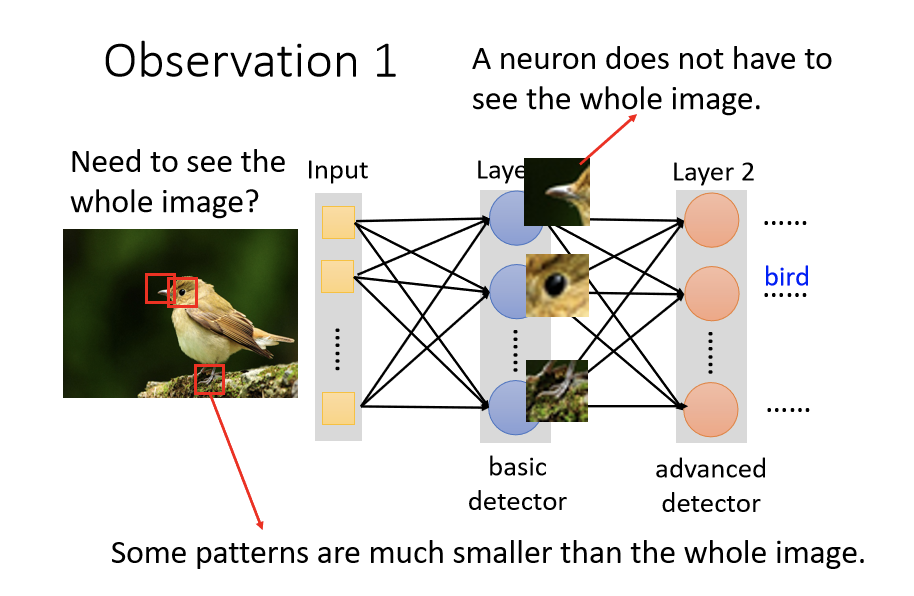
\includegraphics[width=8cm]{picture/PatternDesign.png}
    \caption{Pattern Design}
    \label{fig:galxy}
\end{figure}
\indent 如上图所示,对于某些神经元来说,只需要将图片的一部分作为输入,使它能够检测相应区域的特征有无出现就可以了,因此在下图中给出卷积的相应图示。\par
\indent 在图25中,设定的红框区域称为Receptive Field(感受野),每一个神经元只关注自己的区域,在下图中感受野的区域是\(3 \times 3 \times 3\),也就是27维向量,也就是有27个权重以及一个偏置项。通常所说的kernal size卷积核就是\(3 \times 3\),stride即代表每次卷积核移动的步长,padding代表超出范围时补值的范围。
\begin{figure}[H]
	\begin{minipage}[t]{0.5\linewidth}
		\centering
		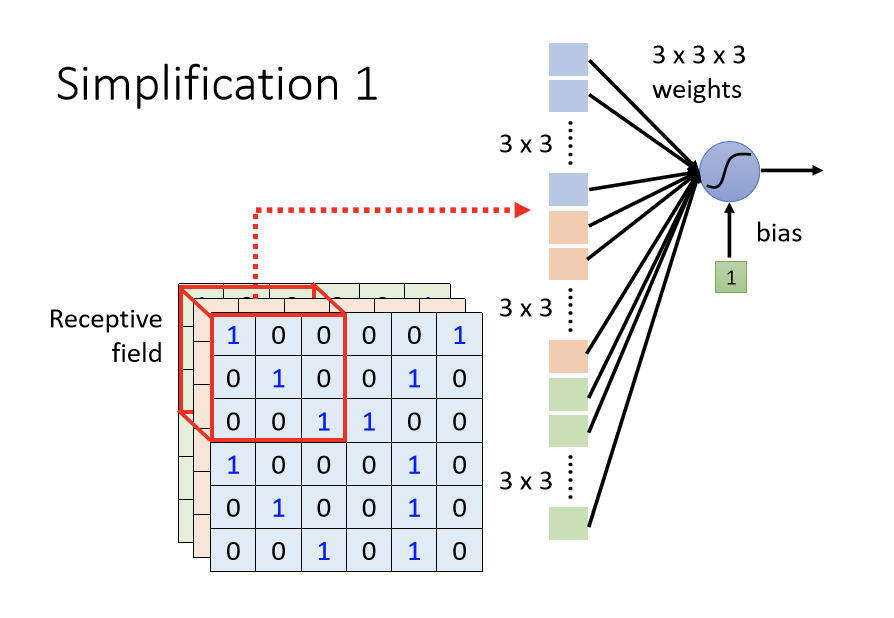
\includegraphics[scale=0.45]{picture/Convolution1.png}
	\end{minipage}
    \quad
	\begin{minipage}[t]{0.5\linewidth}
		\centering
		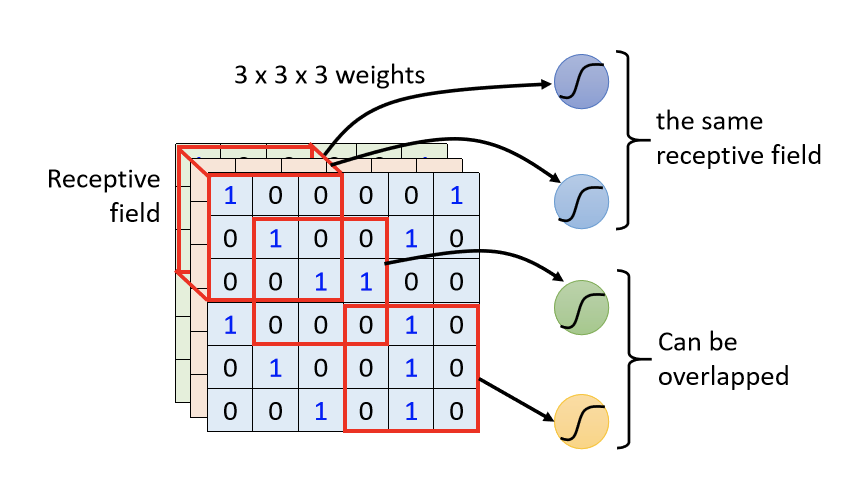
\includegraphics[scale=0.45]{picture/Convolution2.png}
	\end{minipage}
	\\
	\begin{minipage}[t]{0.5\linewidth}
		\centering
		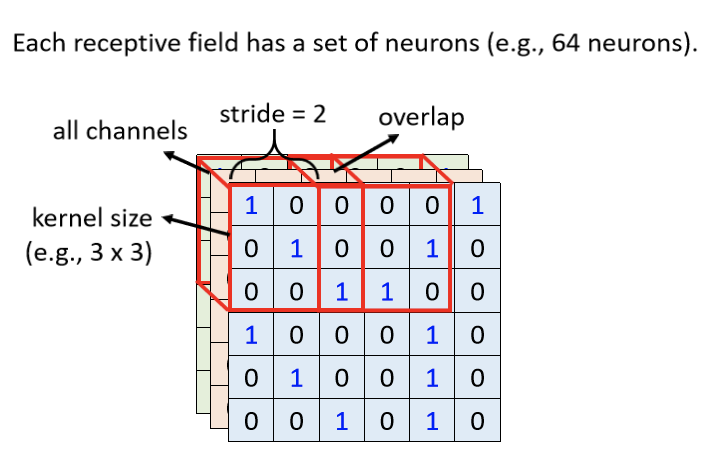
\includegraphics[scale=0.45]{picture/Convolution3.png}
	\end{minipage}
	\begin{minipage}[t]{0.5\linewidth}
		\centering
		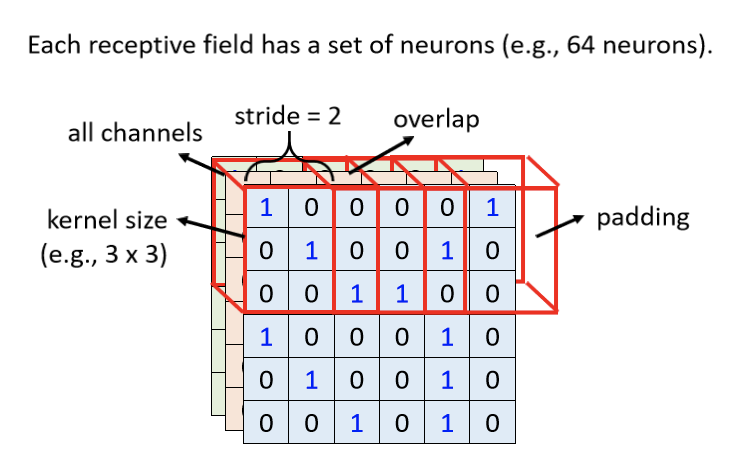
\includegraphics[scale=0.45]{picture/Convolution4.png}
	\end{minipage}
	\caption{Neuron Design}
	\label{fig:galxy}
\end{figure}
\indent 我们可以根据这些参数来确定卷积的运行过程,与此同时给出pytorch中卷积层的代码调用。\par
\begin{lstlisting}
# 卷积层
torch.nn.Conv2d(in_channels, out_channels, kernel_size, 
stride=1, padding=0, dilation=1, groups=1, bias=True, padding_mode='zeros')
\end{lstlisting}

\indent 用更加通俗易懂的方式解释卷积,将考虑一些Filter,即使用Filter对图像进行卷积操作,一个卷积层中有一排的Filter,当使用Filter扫过一张图片,这也就意味着参数共享,即针对每个感受野中的每个位置的相应参数相同。当使用这些Filter扫过图片后,就可以生成FeatureMap,那么生成的FeatureMap可以经过下一层卷积层输出。\par

\begin{figure}[H]
	\begin{minipage}[t]{0.5\linewidth}
		\centering
		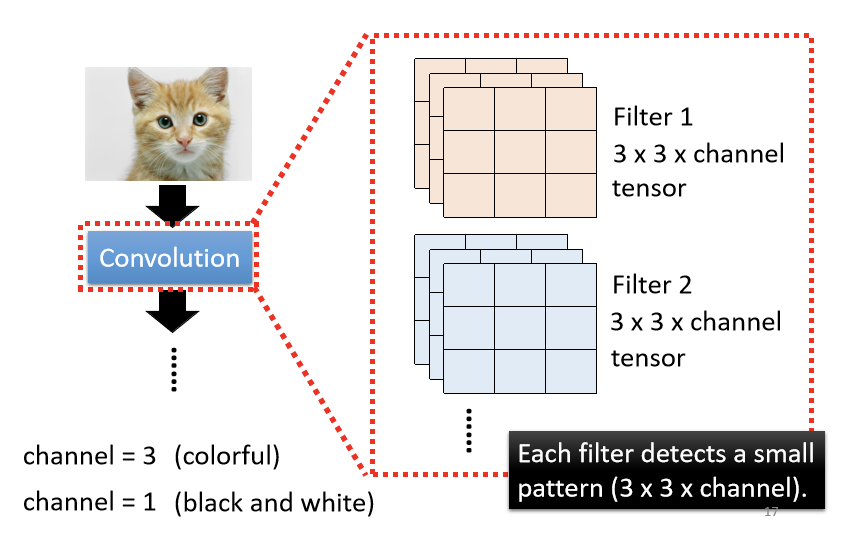
\includegraphics[scale=0.4]{picture/FeatureMap1.png}
	\end{minipage}
    \quad
	\begin{minipage}[t]{0.5\linewidth}
		\centering
		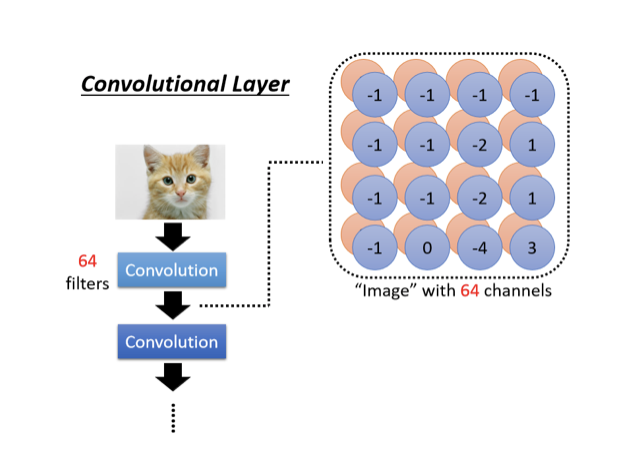
\includegraphics[scale=0.5]{picture/FeatureMap2.png}
	\end{minipage}
	\caption{FeatureMap}
	\label{fig:galxy}
\end{figure}
\indent 在卷积层后,往往会有池化层。也就是Pooling,Pooling的作用主要是将原图像的尺寸缩小,更具体的说就是针对卷积提取到的每个FeatureMap的局部特征进行筛选或融合,选取适当的有代表性的点来表示一个区域,这样做的目的是进行泛化以及降维。 \par
\begin{figure}[H]
	\begin{minipage}[t]{0.5\linewidth}
		\centering
		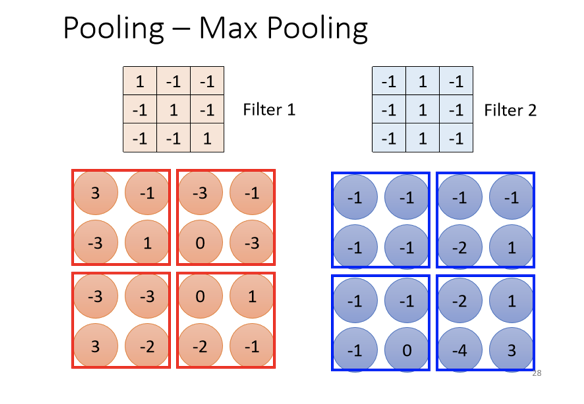
\includegraphics[scale=0.5]{picture/MapPolling1.png}
	\end{minipage}
    \quad
	\begin{minipage}[t]{0.5\linewidth}
		\centering
		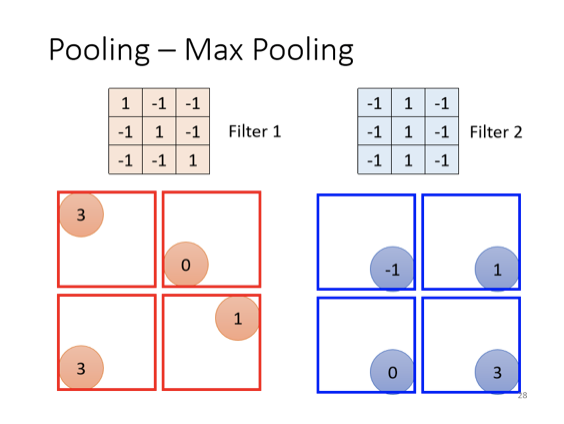
\includegraphics[scale=0.5]{picture/MaxPolling2.png}
	\end{minipage}
	\caption{MaxPooling}
	\label{fig:galxy}
\end{figure}
\begin{lstlisting}
# 池化层
torch.nn.MaxPool2d(kernel_size, stride=None, padding=0, 
dilation=1, return_indices=False, ceil_mode=False)
\end{lstlisting}

\indent 通常来说,经过卷积层、池化层后的维度可以很轻松的确定,但是经过这两层之后的图像的尺寸会比较难确定,因此给出了输入、输出前后图像尺寸大小变换的公式。 \par
\begin{equation}
    \begin{split}
        Height_{out} &= (Height_{in} - Height_{kernal} + 2* padding) / stride + 1\\
        Width_{out}  &= (Width_{in} - Width_{kernal} + 2* padding) / stride + 1
    \end{split}
\end{equation}
\newpage

% -----------------------SECTION 3---------------------
\section{Self-attention}
\indent 记录完了CNN网络结构后,将记录另一个较为常见的网络架构,即Self-Attention,通常称为自注意力模型。考虑输入一串语句,那么如何将它们进行联系起来,首先介绍一下Word Embedding,该策略将会给输入的每一个词汇一个向量,该向量会带有一定的语义资讯,而一个句子就是一排长度不一的向量。假设我们使用全连接层作为网络模型,那么我们输入一段文本文字,例如含有相同单词但是不同意思的文本,对于全连接层网络来说,相同单词它会输出相同的东西,而我们所期望的是网络能够根据上下文信息来学习输出,因此就需要Self-Attention。  \par

\begin{figure}[H]
    \centering
    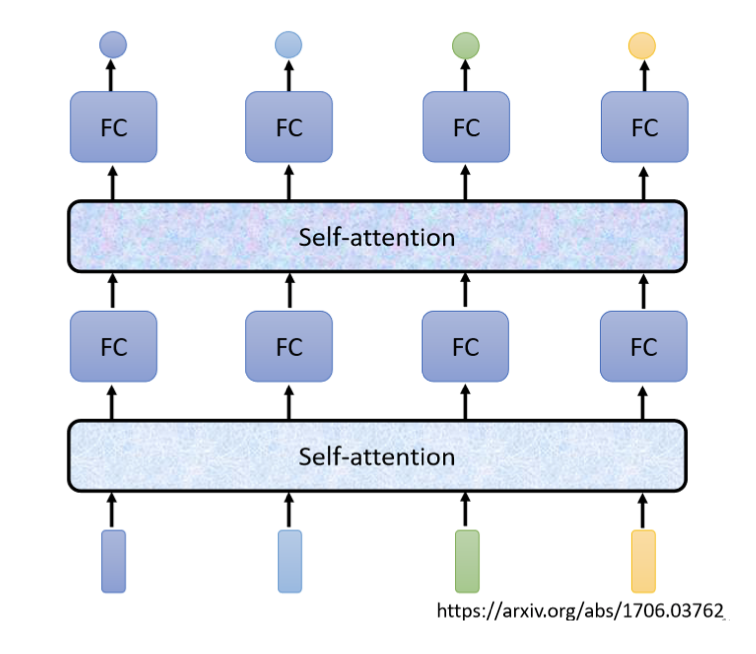
\includegraphics[width=8cm]{picture/SelfAttention.png}
    \caption{Self-Attention}
    \label{fig:galxy}
\end{figure}

\indent 上面给出了一些使用Self-Attention的网络模型架构,在Self-Attention中,输入和输出的数量相同,且其输出的向量都是考虑整个输入序列的咨询而产生的。并且可以把Self-Attention与全连接层交替使用,Self-Attention处理整个输入序列的资讯,而全连接层专注于处理某一个位置的资讯处理。 \par
\indent 接着将会记录一下Self-Attention的整个过程,假设Self-Attention的输入输出均为4个,如下图所示。

\begin{figure}[H]
    \centering
    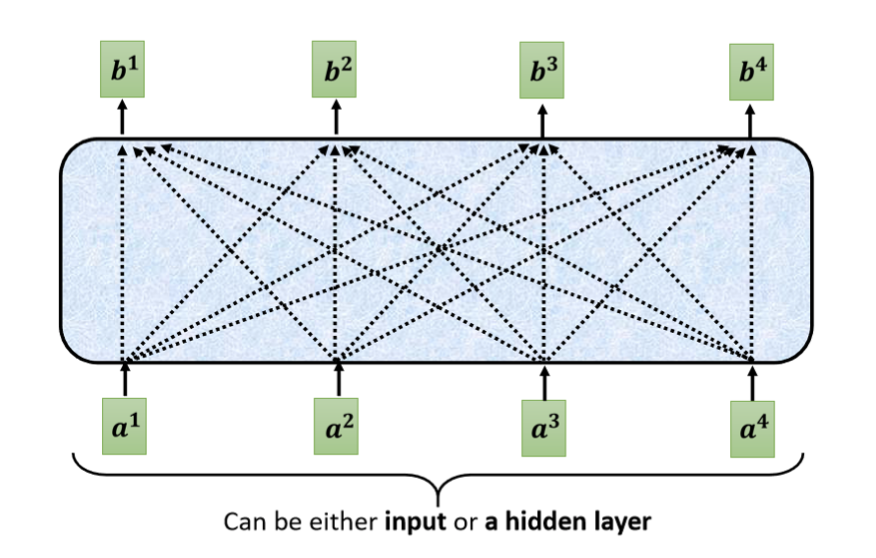
\includegraphics[width=8cm]{picture/SelfAttention1.png}
    \caption{Explanation of Self-Attention}
    \label{fig:galxy}
\end{figure}

\indent 每一个b均考虑了所有a才产生出来,并且同时将会考虑输入序列中其他向量与\(a^{1}\)的关联度,那么如何计算它们的关联度\( \alpha \)呢,因此就需要计算attention的模组。  \par

\begin{figure}[H]
	\begin{minipage}[t]{0.5\linewidth}
		\centering
		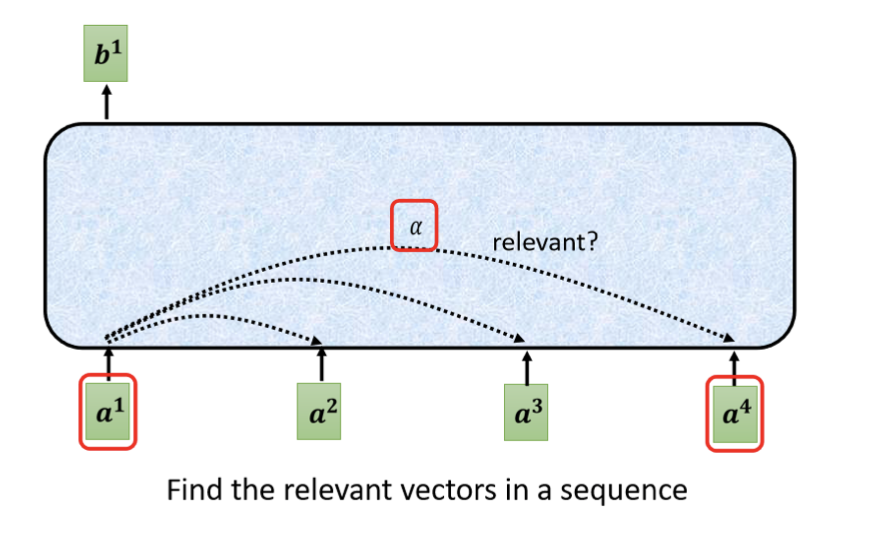
\includegraphics[scale=0.4]{picture/SelfAttention2.png}
	\end{minipage}
    \quad
	\begin{minipage}[t]{0.5\linewidth}
		\centering
		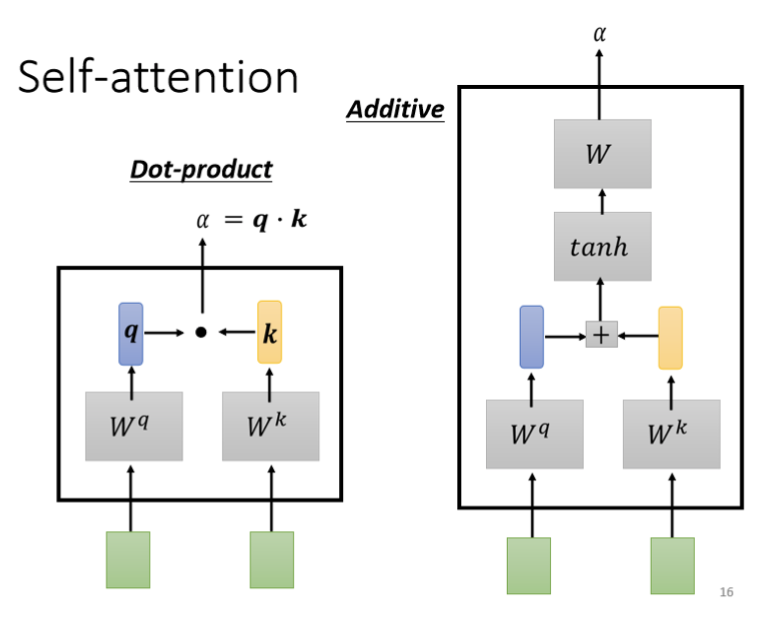
\includegraphics[scale=0.4]{picture/SelfAttention3.png}
	\end{minipage}
	\caption{Computation of Self-Attention}
	\label{fig:galxy}
\end{figure}

\indent 而计算attention最常用的方式就是dot-product,其主要的计算方法就是\(q^{1} = a^{1}W^{q} \),其中通常称\(q\)为Query,而对于\(a^{2}、a^{3}、a^{4}\)乘以\(W^{k}\)则会得到\(k\),通常称之为Key,最后计算attention分数\(\alpha_{i,j}=q^{i}k^{j}\),值得注意的是,往往也会计算自关联,并且在计算出attention分数后(即计算出关联性后),往往会添加一层softmax。并将\(a^{1}\)到\(a^{4}\)的输入向量乘上\(W^{v}\)得到新的\(v^{1}v^{2}v^{3}v^{4}\)向量,最后将得到的向量与softmax层的输出像乘,得到\(b^{i}\),也就是Self-Attention的输出。 \par
\indent 可以发现,在Self-Attention中,较为重要的是\(W^{q}、W^{k}、W^{v}\)三个参数,这些参数是需要通过训练来拟合的。 \par

\begin{figure}[H]
    \centering
	\subfigure[]{
	    \begin{minipage}[b]{0.7\textwidth}
	        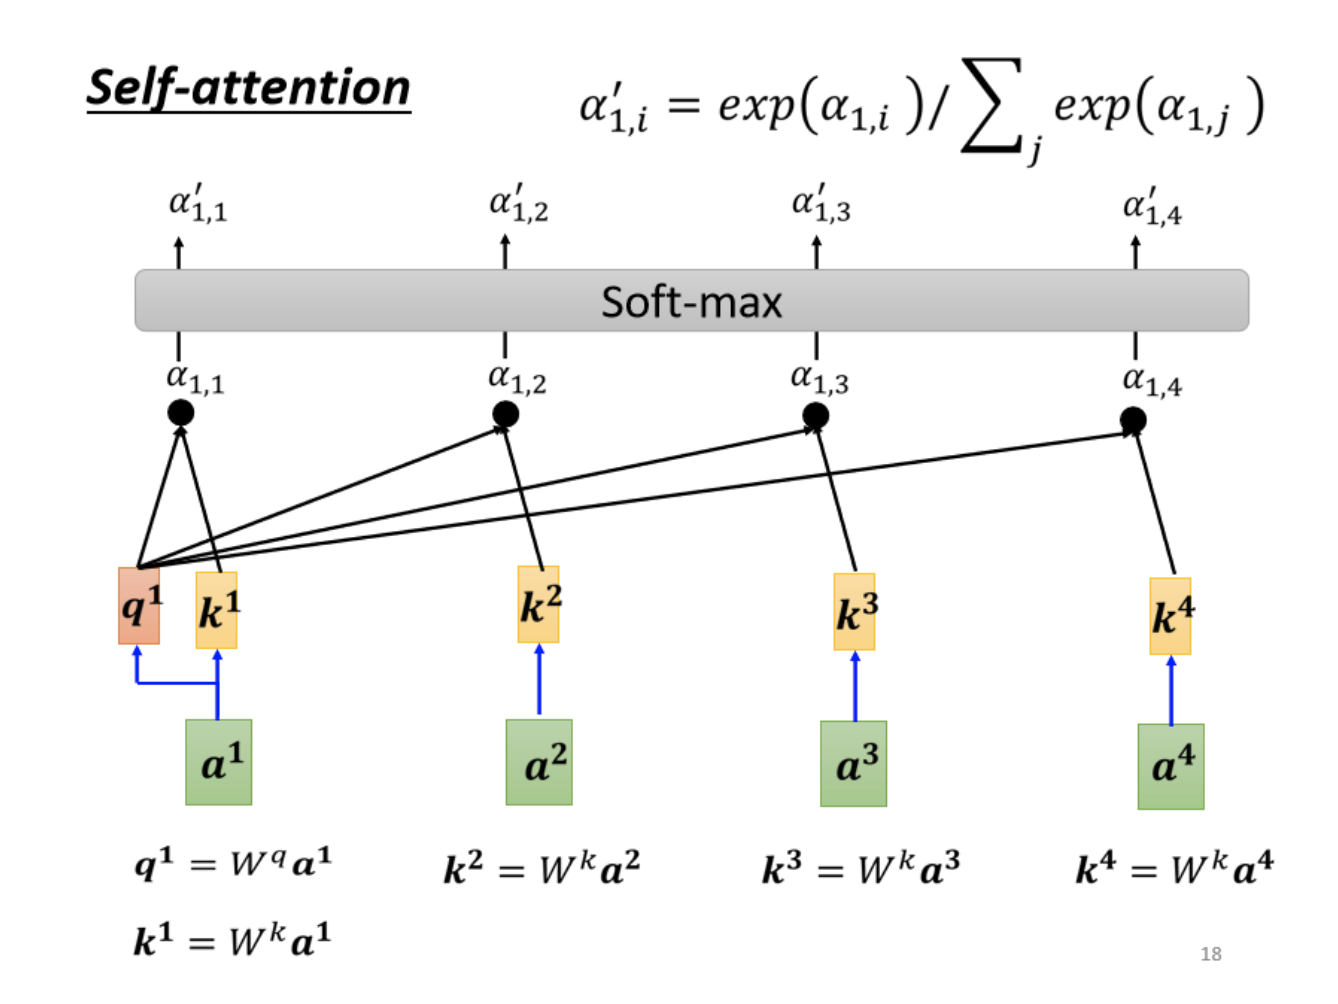
\includegraphics[width=1\textwidth]{picture/SelfAttention4.png}
	    \end{minipage}
	}
	\subfigure[]{
	    \begin{minipage}[b]{0.7\textwidth}
	        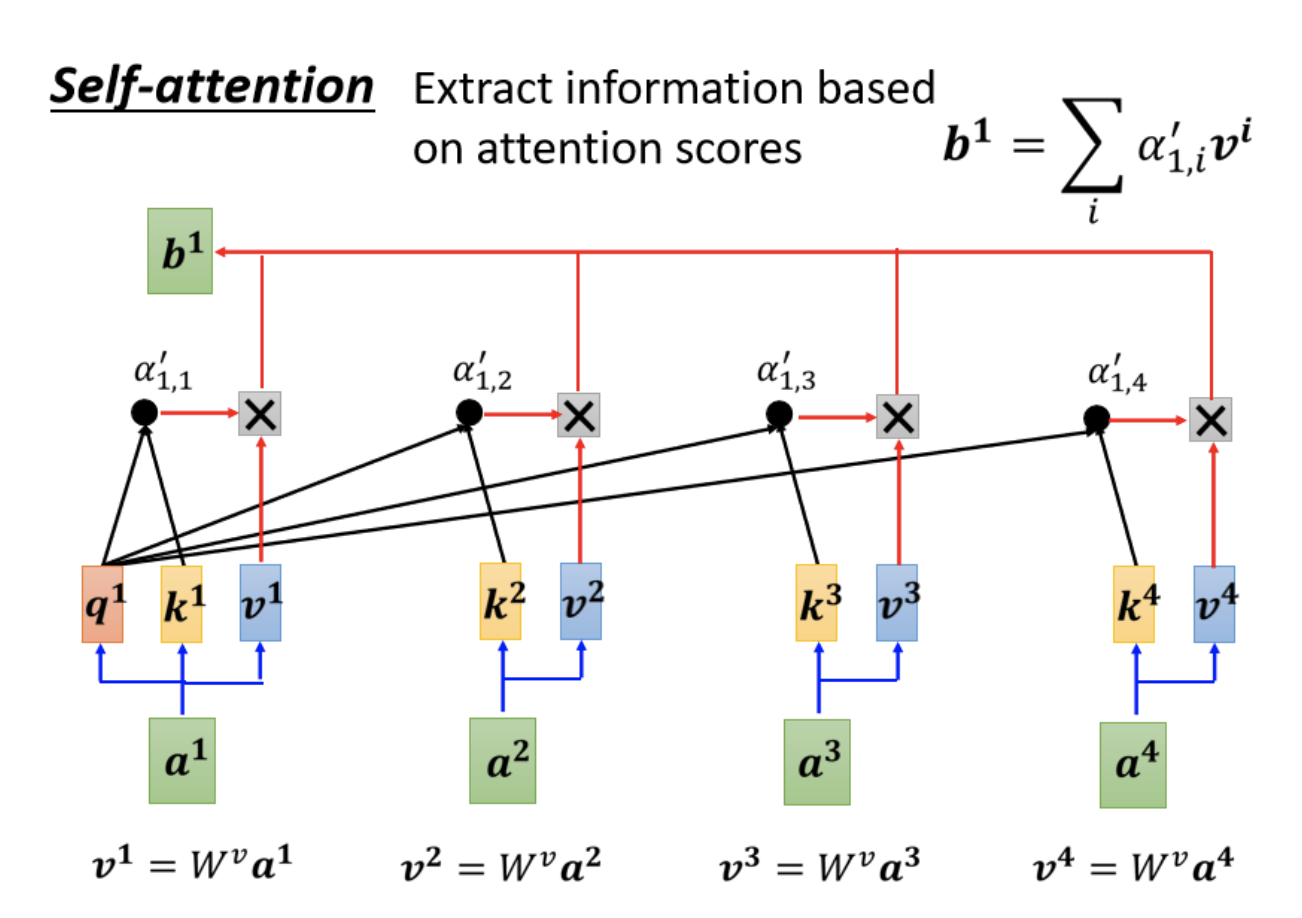
\includegraphics[width=1\textwidth]{picture/SelfAttention5.png}
	    \end{minipage}
	}
	\caption{Computation of Self-Attention}
	\label{fig:galxy}
\end{figure}

\indent 接下来则会简要的记录一下Multi-head Self-Attention,相比于普通的Self-Attention,该网络模型的变化则是增加参数来计算更多的相关性。简单来说就是增加一层\(W^{q}、W^{k}、W^{v}\)参数而已。 \par
\begin{figure}[H]
    \centering
    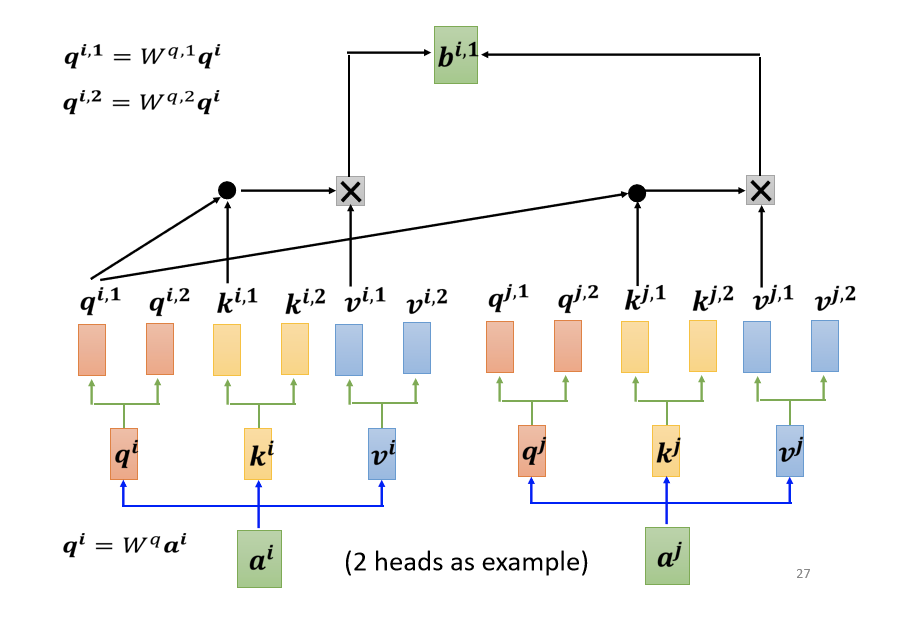
\includegraphics[width=8cm]{picture/MultiHeadAttention.png}
    \caption{Pattern Design}
    \label{fig:galxy}
\end{figure}

%---------------------------SECTION4------------------------------
\section{Transformer}
\indent Transformer是变形金刚的英文,而Transformer模型的特点也和其有些相似,因此将在这一章记录有关Transformer相关的知识要点。 \par
\indent Transformer是Sequence-to-Sequence的模型,其通常写作Seq2seq,序列到序列的模型顾名思义,输入是序列,输出也是序列。更加具体的解读则是输入一段序列,输出序列的长度及内容由模型预测而给出。\par
\begin{figure}[H]
    \centering
    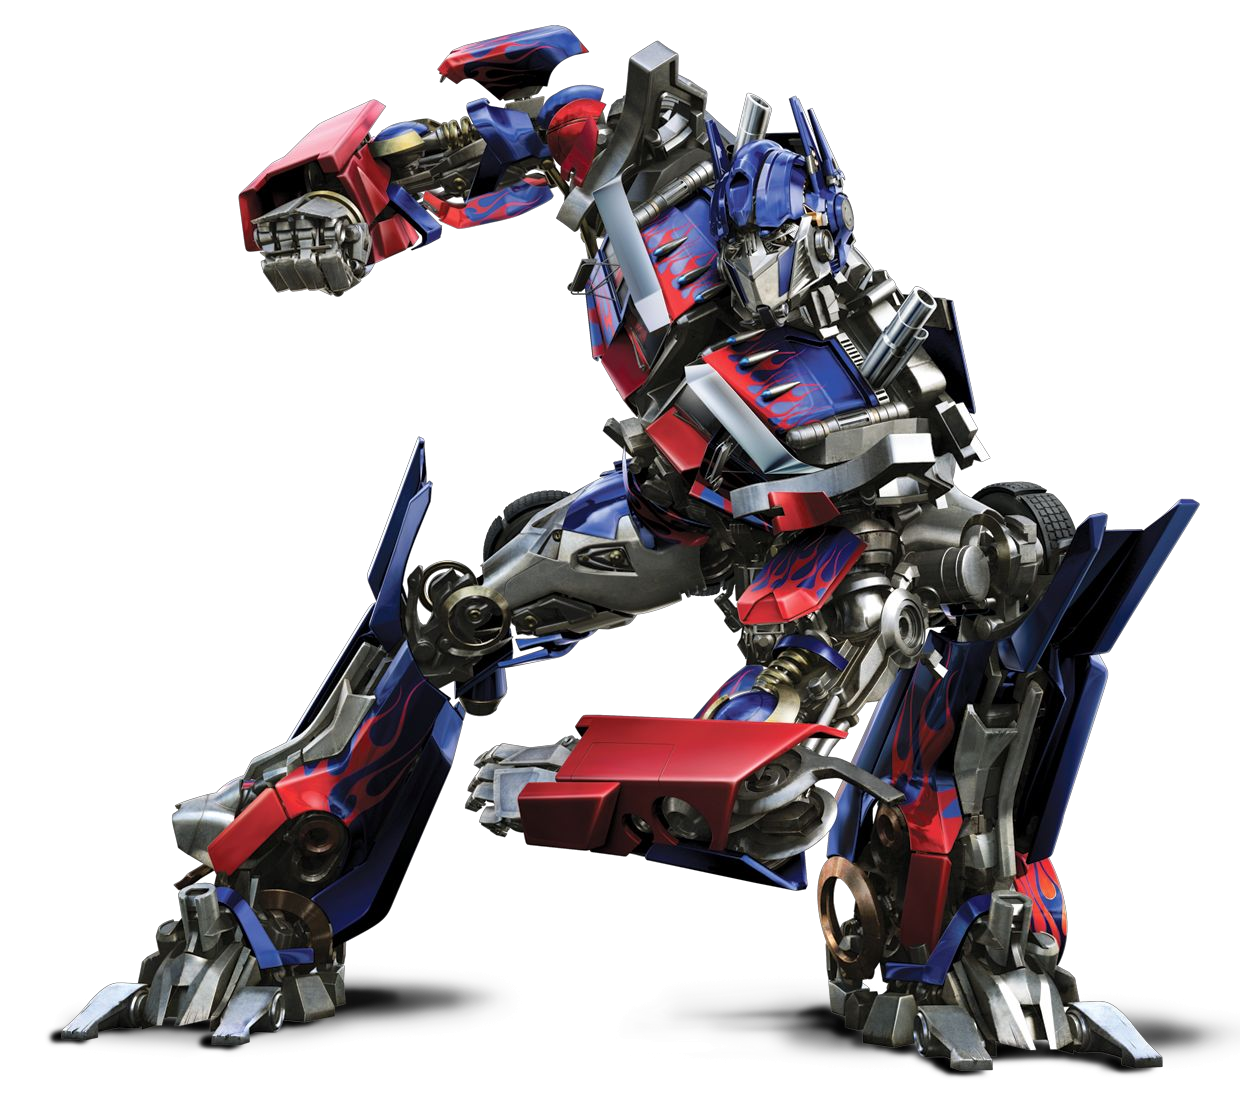
\includegraphics[width=6cm]{picture/Transformers.png}
    \caption{Transformer}
    \label{fig:galxy}
\end{figure}
\indent 一般在Seq2seq的模型中,一般会分为两块,一块是Encoder,另一块则是Decoder,Transformer中泽有一个Encoder架构以及一个Decoder架构,接下来会在两节中记录这两种结构的处理细节。 \par
\begin{figure}[H]
    \centering
    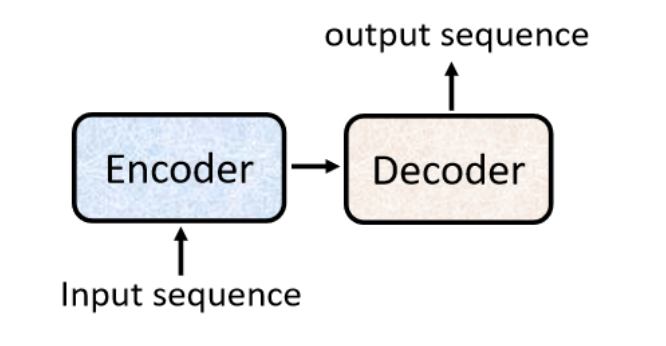
\includegraphics[width=8cm]{picture/EDcoder.png}
    \caption{Encoder-Decoder}
    \label{fig:galxy}
\end{figure}

\subsection{Encoder}
\indent 首先将会从总体来介绍Encoder的结构,具体如下图所示,Encoder所需要做的事情就是输入一排向量并输出另一排向量,因此许多模型都可以做到,例如RNN、CNN,在Transformer中的Encoder则是使用Self-Attention。Encoder的结构如下图所示。 \par
\begin{figure}[H]
    \centering
    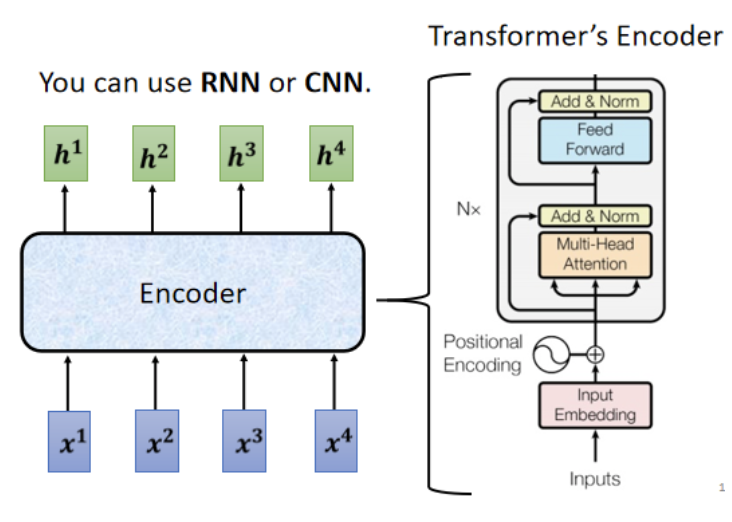
\includegraphics[width=8cm]{picture/Encoder.png}
    \caption{Encoder Architecture}
    \label{fig:galxy}
\end{figure}
\indent 在Encoder中,往往会分成很多个block,每一个block由多个神经网络层组,举例来说买,一个block可以由一层Self-Attention以及一层全联接层组成。 \par
\begin{figure}[H]
    \centering
    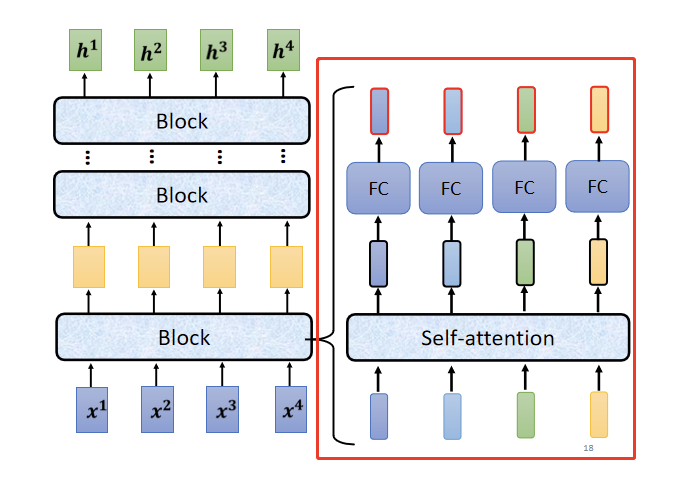
\includegraphics[width=8cm]{picture/EncoderBlock.png}
    \caption{Encoder Block}
    \label{fig:galxy}
\end{figure}
\indent 而在Transformer中,block往往会比较复杂,如下图所示。在经过Self-Attention后得到输出向量,在Transformer中,不只是输出vector,还要将输入拉过来加给输出,得到新的Output。其实这种网络架构称为residual connection,得到输出后再对其进行标准化(normlization)。 \par
\begin{figure}[H]
    \centering
    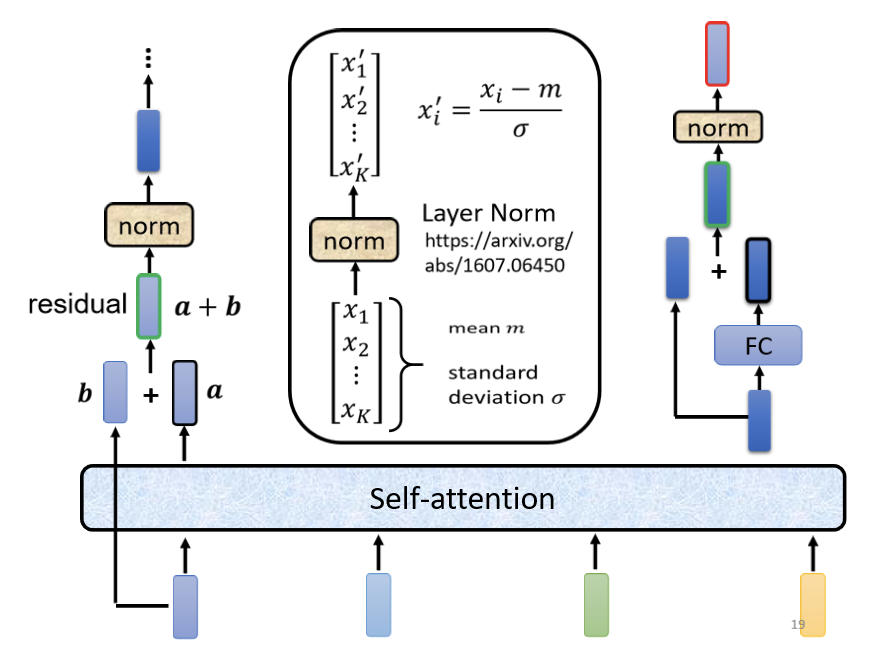
\includegraphics[width=8cm]{picture/EncoderSelfAttention.png}
    \caption{Encoder Self-Attention}
    \label{fig:galxy}
\end{figure}
\indent 这边给出layer normalization的公式。相同的,针对全连接层,也同样可以使用残差架构以及标准化来得到输出,最后再看图35,可以发现Transformer的encoder所做的就是这些事情。 \par
\begin{equation}
    x^{\prime}_{i} = \frac{x_{i}-m}{\sigma}
\end{equation}
\indent 这边给出layer normalization的公式。相同的,针对全连接层,也同样可以使用残差架构以及标准化来得到输出,最后再看图35,可以发现Transformer的encoder所做的就是这些事情。 \par

\subsection{Decoder}
\indent Decoder主要分为两种,第一种是Autoregressive(AT),另一种是Non-autoregressive(NAT),比较常见及经常使用的是AT。由上节可知,Encoder的作用是输入一串向量,输出一串向量,而Decoder就是将输出向量作为输入得到最终的结果。\par
\begin{figure}[H]
    \centering
    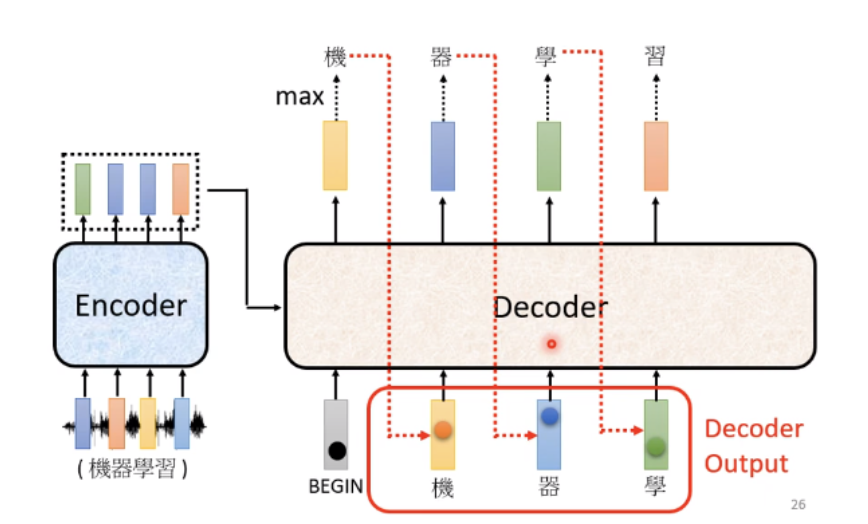
\includegraphics[width=8cm]{picture/DecoderOutput.png}
    \caption{Decoder }
    \label{fig:galxy}
\end{figure}
\indent 从上图可知,Decoder会接收Encoder的输入,也会把自己的输入当作接下来的输出,并且在下图也会给出Transfomer的Decoder结构,其实可以发现,相比于Encoder,Decoder比较不同的方面就是多了一个Masked Multi-head Attention以及最后输出的线形、softmax层。
\begin{figure}[H]
    \centering
    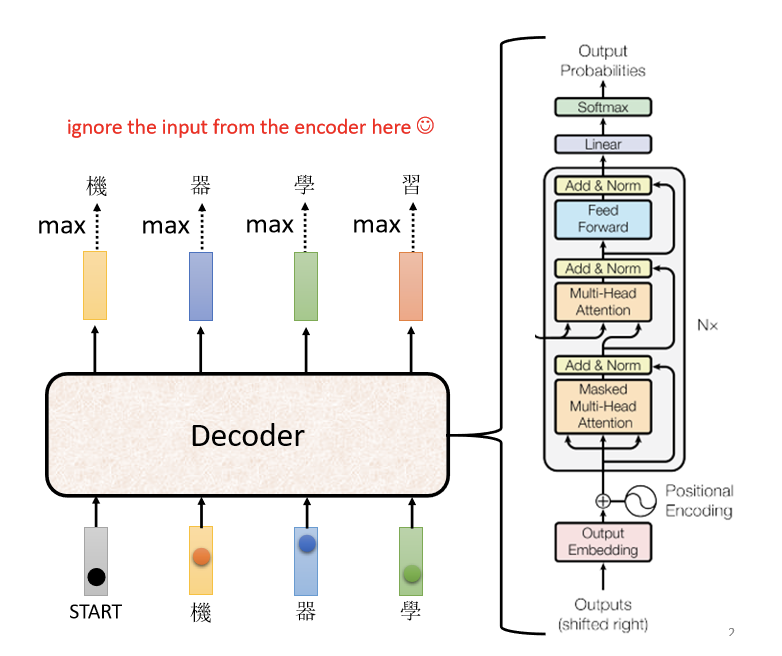
\includegraphics[width=8cm]{picture/DecoderArchitecture.png}
    \caption{Decoder Architecture}
    \label{fig:galxy}
\end{figure}
\indent 而加入Masked与不加Masked的区别则是考虑到Decoder的运作方式,它是一个一个输出,所以先有\(a^{1}\)再有\(a^{2}\)......因此在Masked Multi-head Attention中计算关联Attention分数的时候,只将当前的输入向量与前面的向量进行计算操作,而不与后面的向量计算分数。具体如下图所示。\par
\begin{figure}[H]
    \centering
    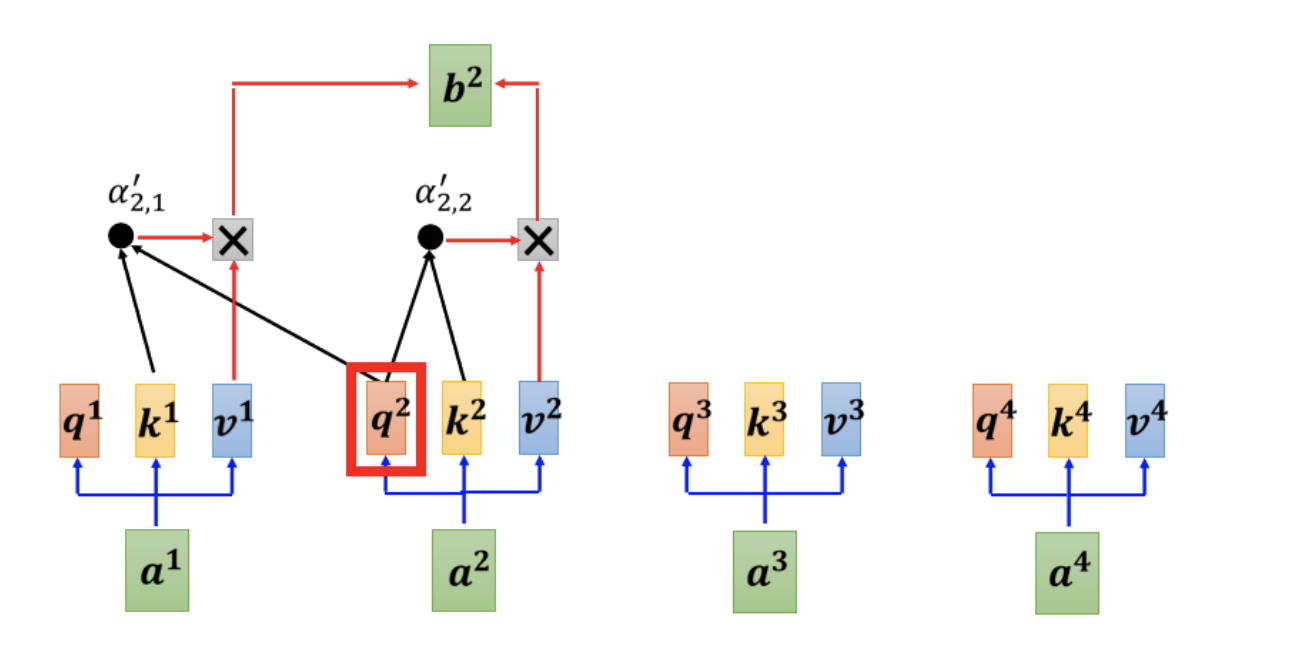
\includegraphics[width=8cm]{picture/MaskedMulti-headAttention.png}
    \caption{Masked Multi-head Attention}
    \label{fig:galxy}
\end{figure}
\indent Decoder中还有一个关键的问题则是它会自己推断输出的序列长度,因此它需要考虑什么时候结束输出,通常在输出预测中会有一个end符号,当模型输出end时则代表输出结束。 \par

\subsection{Encoder-Decoder}
\indent 在分别记录了Encoder结构以及Decoder的结构之后,则需要考虑Encoder与Decoder的是如何连接的,这里给出Transformer的整个结构,其中连接的部分被框出,其被称为Cross Attention,其中有两个输入来自Encoder,Decoder提供一个输入。 \par
\begin{figure}[H]
    \centering
    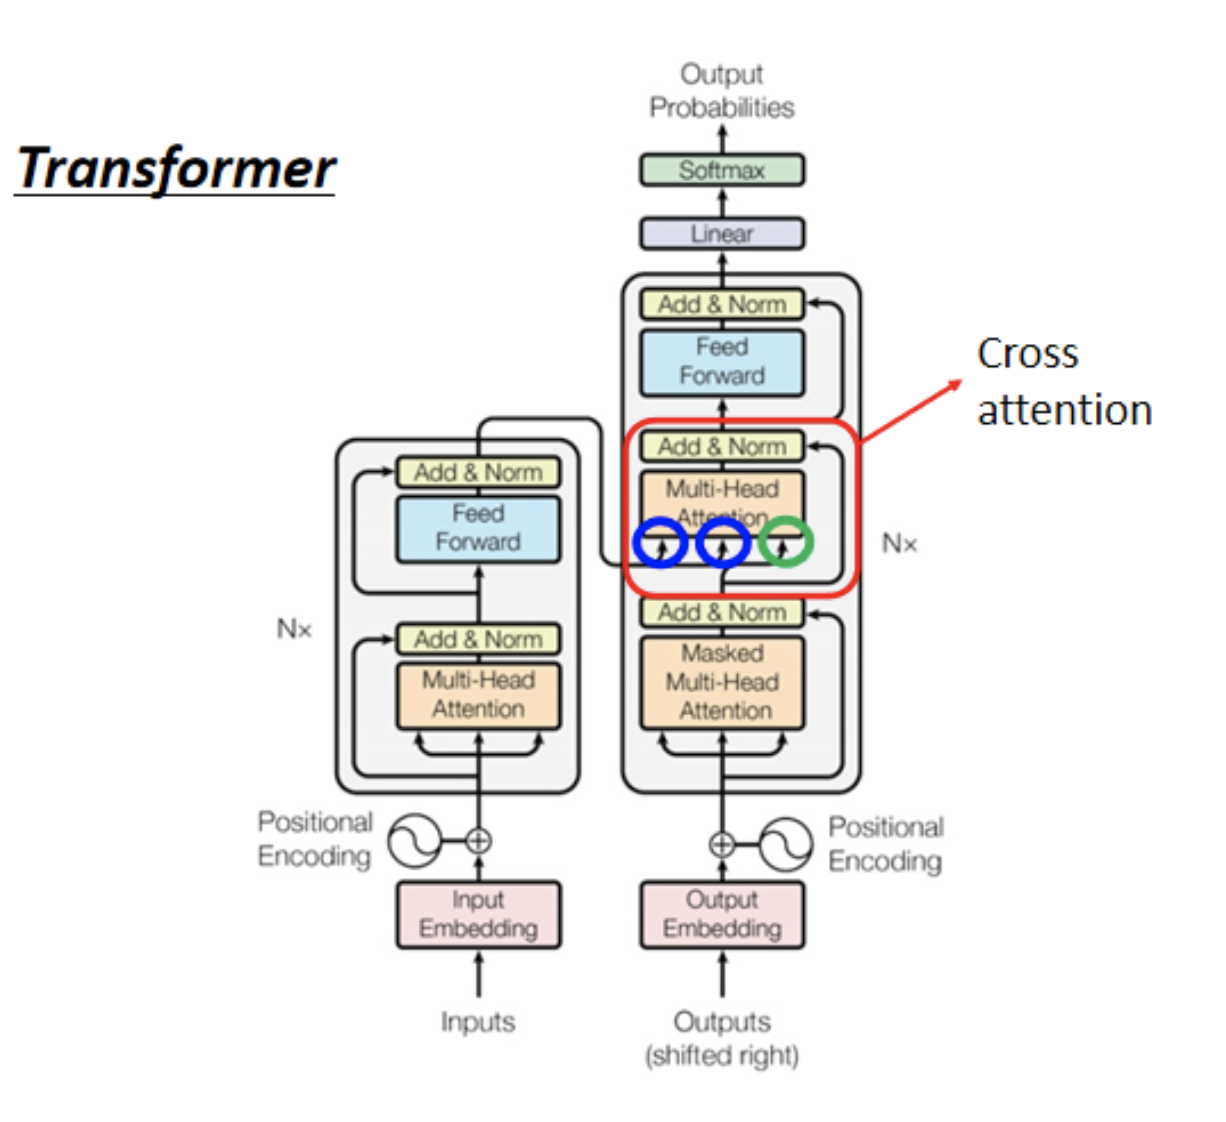
\includegraphics[width=8cm]{picture/Encoder-Decoder.png}
    \caption{Transformer Architecture}
    \label{fig:galxy}
\end{figure}
\indent Cross Attention的具体运作形式如下图所示,简单来说是将Encoder的输出向量与Decoder的经过一部分变换的输出(Masked Multi-Head Attention + Add + normalization),对应于图41,q来自于Decoder,k、v来自Encoder,交叉计算attention。 \par
\begin{figure}[H]
    \centering
    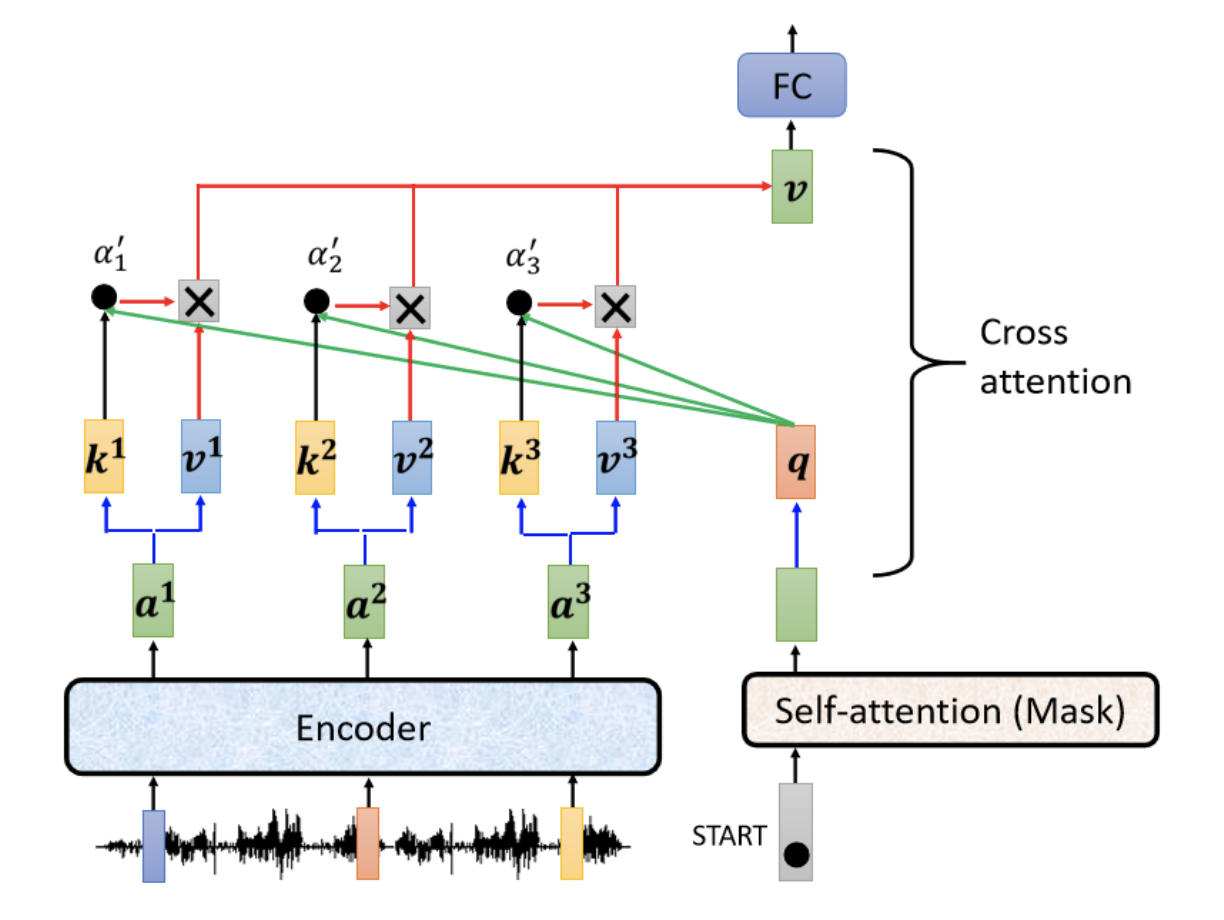
\includegraphics[width=8cm]{picture/CrossAttention.png}
    \caption{Cross Attention}
    \label{fig:galxy}
\end{figure}
\indent Transformer的整体构造还是有些复杂的,更多的训练细节需要在论文中阅读理解。
% -----------------------------SECTION5----------------------------
\section{To Learn more}
\indent 至此,已经了解了几个在视觉领域比较基础重要的网络结构,但是课程中涉及更多的是网络结构的设计理解,而更多的小细节需要从论文中去获取,与此同时也需要去复现一些经典论文在实践中提升自己对网络架构的理解。因此按照年份列举一些比较重要的网络结构,以及下图课程中所提到的。将会在下面列出一些网络结构的论文网址 \par
\begin{figure}[H]
    \centering
    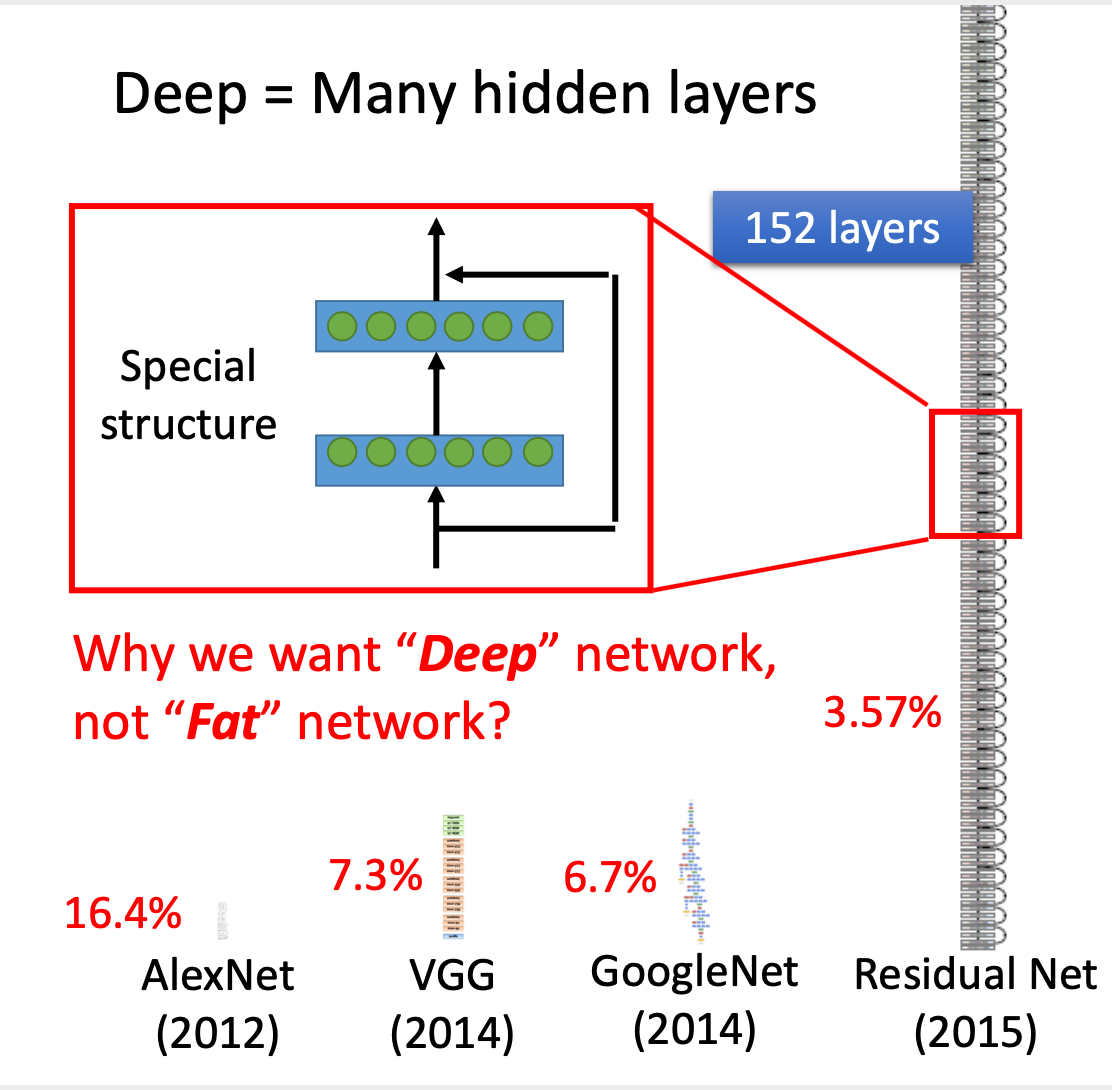
\includegraphics[width=8cm]{picture/TipycalNeuralNetwork.png}
    \caption{Tipycal Neural Network}
    \label{fig:galxy}
\end{figure}

\noindent AlexNet : \url{https://proceedings.neurips.cc/paper/2012/file/c399862d3b9d6b76c8436e924a68c45b-Paper.pdf} \par
\noindent VGG : \url{https://arxiv.org/abs/1409.1556} \par
\noindent GoogLeNet : \url{https://arxiv.org/abs/1409.4842} \par
\noindent ResNet : \url{https://arxiv.org/abs/1512.03385}\par
\noindent R-CNN : \url{https://arxiv.org/abs/1311.2524}\par
\noindent Faster R-CNN : \url{https://arxiv.org/abs/1506.01497}\par
\noindent Transformer : \url{https://arxiv.org/abs/1706.03762}\par

\end{document}
